% !TeX program = lualatex
\documentclass[mres, greychapternumbers]{mqthesis}
%----------------------------------------------------------
% OPTIONS
% Options you can use in the documentclass above:
%
% phd/mres/hons = set the degree text [default=phd]
% copyrightpage = print a copyright page on the back 
%                 of the title page [default=false]. 
%		NOTE: if true, you will have to manually change the name
%		            and date in the mqthesis.cls file.
% examinerscopy = print "Examiner's Copy" of title page and 
%                 change linespacing to 1.5 [default=false]
% greychapternumbers = print large chapter numbers in grey
%                 instead of MQ corporate "sand"
%---------------------------------------------------------- 

% this shows what labels you are using for cross references
% \usepackage{showkeys} 
\usepackage{helvet}
% ifthenelse for if loops
\usepackage{etoolbox}
\usepackage{amsmath}
\usepackage{amsfonts}
\usepackage{amssymb}
\usepackage{graphicx}
\usepackage{float}
\graphicspath{ {images/} }
\usepackage{algorithm}
\usepackage{algpseudocode}
\algdef{SE}[SUBALG]{Indent}{EndIndent}{}{\algorithmicend\ }
\algtext*{Indent}
\algtext*{EndIndent}
\usepackage{natbib}
\usepackage{bm}
\usepackage{hyperref}
\usepackage{svg}
%\usepackage{bbm}
\usepackage[most]{tcolorbox}
\usepackage{tikz}
\usepackage{pgfplots}
  \pgfplotsset{compat=newest}
\newlength\fheight
\newlength\fwidth
\usepackage{csquotes}
\raggedbottom

\usepackage{multicol}
\setlength{\columnsep}{0.5cm}

\newcommand{\mathbbm}[1]{\text{\usefont{U}{bbm}{m}{n}#1}}

\AtBeginEnvironment{tcolorbox}{\footnotesize\linespread{1}\selectfont}

\linespread{1.3}\selectfont

%---------------------------------------------------------
% SPECIFIC OPTIONS
% Other options to use in this thesis:
%
% smallcapschapter = use smallcaps for chapter titles
\newtoggle{smallcapschapter}
\togglefalse{smallcapschapter} % Change to true if you want capitals for chapter titles/headings
%----------------------------------------------------------



%---------------------------------------------------------- 
% STRUCTURE
% this document is a skeleton which pulls in the meat of the thesis
% from other files. Comment out and add lines as appropriate.
%---------------------------------------------------------- 


\begin{document}

%---------------------------------------------------------- 
% FRONT
% Acknowledgements, titlepage, abstract, list of publications
%---------------------------------------------------------- 
\frontmatter

\title{Approximate Bayesian Tomography} % put your title here
\author{Thomas Connell} % put your name here
\department{Earth and Planetary Sciences}  % put your department here
\submitdate{14th October 2018}

\titlepage

\chapter{Acknowledgements}

I would like to ackowledge the love and support of Melanie. Without it this work would not have been possible.\\ 

I would also like to thank the continuous encouragement from my parents Sean and Heather, who always pushed me to do what I wanted. Without such freedom I may never have ended up on the path I am now.
 % acknowledgements (acknowledge.tex)
\chapter{Abstract}

%Geophysical inverse problems open up the interior of the Earth. Their solution describes the inner working of our planet. The methods of inverse problems are a continually evolving field, fed by breakthroughs in mathematics. Recently, probabilistic solutions have been advocated for in geophysics. Probabilistic tomography can tackle the inherit non-uniqueness of the model space and the uncertainty in both data and modelization. This formulation depends on traditional likelihood machinary. By extension, it also suffers from the limiting aspects and assumptions which are implicit in the construction of a likelihood function. Here I explore the geophysical applicability of likelihood-free probabilistic methods, coined Approximate Bayesian Computation (ABC) in the statistics literature. ABC offers the chance to build upon the progress in probabilistic tomography and overcome downfalls which result from the formalism of likelihood based tomography.\par
Geophysical \textit{inverse problems} define Earth's structure based on experiental observations. Their solution is an invaluable line of evidence to scrutinize hypotheses about our planet. Recently, to quantify uncertainty in the experimental observations and the \textit{forward problem}, explore trade-offs between model parameters and constrain the solution with a priori information, probabilistic methods for inverse problems have been pioneered in geophysics. While traditional linear methods are weakened under these conditions probabilistic methods based on a Bayesian formulation are well suited.  There are, however, implicit assumptions in the construction and use of the likelihood function in Bayesian inference. Here I scrutinize these assumptions and advocate for the use of likelihood-free Bayesian inference, coined Approximate Bayesian Computation, as a method which can build upon the success of probabilistic tomography. Here I show that Approximate Bayesian Computation can utilize the information available in a dataset to drive rapid convergence to low misfit models while maintaining formal statistical guarantees. Efficient algorithms of this kind are required for probabilistic methods to tackle the scale and complexity of large inverse problems about Earth’s deep internal structure. By freeing inference from the limiting aspects of a likelihood function, Approximate Bayesian Computation promises to expand parameter inference to problems which were previously intractable. \par
This thesis is a 9 month study, undertaken from January 5 - October 14 2018. 
 % abstract (abstract.tex)

\linespread{1}\selectfont
\tableofcontents 
% comment out these as required for your discipline
\listoffigures
\listoftables

%---------------------------------------------------------- 
% MAIN
% include chapters as needed
%---------------------------------------------------------- 
\mainmatter

\makeatletter
\let\old@makechapterhead\@makechapterhead
%----------------------------------------------------------
% Use old school chapter headers
% This uses less space, but may not strictly follow
% the MQ style.
% Comment/uncomment out the following
%----------------------------------------------------------
\makeatletter
\def\thickhrulefill{\leavevmode \leaders \hrule height 1ex \hfill \kern \z@}
\def\@makechapterhead#1{%
  {\parindent \z@ \raggedright
    \reset@font
    \hrule
    \vspace*{10\p@}%
    \par
    \iftoggle{smallcapschapter}{  %SRM: Control smallcaps chapter titles
   	 \Large \sc \@chapapp{} \Huge\bfseries \thechapter
	}{
	\Large \@chapapp{} \Huge\bfseries \thechapter
	}
    \par\nobreak
    \vspace*{10\p@}%
    \hrule
    \par
    \vspace*{1\p@}%
    \hrule
    %\vskip 40\p@
    \vspace*{20\p@}
    \Huge \bfseries #1\par\nobreak
    \vskip 20\p@
  }}
%----------------------------------------------------------
% Use old school chapter headers
% This uses less space, but may not strictly follow
% the MQ style.
% Comment/uncomment out the previous
%----------------------------------------------------------

\linespread{1.3}\selectfont

% Introduction
\chapter{Introduction}


\section{Statement of Aims} 

This body of work is concerned with the methods of \textit{inverse problems} \citep{Tarantola2005,Aster2013,Menke2012,Kaipio2006,Biegler2010,Idier2013}. Inverse problems are also referred to as parameter inference or parameter estimation \citep{Box1973,Sprott2008,Casella1993,Cox2007}. Model parameter inference based on observable data is a pursuit which transcends scientific disciplines. For geophysics it is the most important method which allows data to be transformed from surface observations into subsurface images. The effectiveness of traditional methods of geophysical parameter inference is limited when characterizing non-linear systems with trade-offs between parameters and inherit non-uniqueness. Under these conditions probabilistic parameter inference has demonstrated utility in imaging the subsurface \citep{Tarantola2005}. With that in mind, this project seeks to explore the geophysical applicability of a recently developed method of probabilistic parameter inference, known as \underline{A}pproximate \underline{B}ayesian \underline{C}omputation, (ABC), which has emerged from applied challenges in genetics \citep{Tavare1997,Beaumont2002,Sunnaker2013}. This project was started on January 5th, 2018 and concluded with the submission of this document on the 14th of October, 2018. All codes used in this project are written by the author and available at \url{https://github.com/tomconnell/abc-toy-problems} and \url{https://github.com/tomconnell/approximate-bayesian-tomography}.

\section{Parameter inference}

For geophysics, the unknown parameters, $\bm{\theta} = \{\theta_1,...,\theta_N\}$, for a causative model, $\mathcal{M}$, are sought based on observed data, $\bm{y} = \{y_1,...,y_M\}$. The relationship between model parameters and data may be highly non-linear and is represented through the operator $\bm{g}$:
\begin{equation}
\bm{y} = \bm{g}(\bm{\theta})
\label{basic_data_parameters}
\end{equation}
In geophysics we are interested in defining the physical properties  of the subsurface (e.g. seismic velocity, density) from experimental data, $\bm{y}$, observed at the surface (e.g. seismic signals, gravitational acceleration). Deterministic physical models, $\mathcal{M}$, link a parameterized subsurface model to simulated data, $\bm{y'}$. Imaging the subsurface collapses to a parameter inference problem \citep[p.1-2]{Tarantola2005}.\par

Geophysical parameter inference belongs to a large class of problems known as \textit{inverse problems} \citep{Tarantola2005,Aster2013,Menke2012}. These methods use experimental data, $\bm{y}$, to infer the causative model parameters, $\bm{\theta}$. This contrasts with the \textit{forward problem}, which starts with a given set of model parameters, $\bm{\theta'}$, and produce a set of simulated data, $\bm{y'}$. Both areas are subject to considerable research and development. The ability to solve the forward problem is required to solve the inverse problem.
\begin{equation}
\text{The inverse problem:}\ \bm{y} \rightarrow \bm{\theta}
\label{inverse_problem}
\end{equation}
\begin{equation}
\text{The forward problem:}\ \bm{\theta'} \rightarrow \bm{y'}
\label{forward_problem}
\end{equation}


\section{Probabilistic formulation}

Geophysical inverse problems come with a unique set of challenges. Often the experimental data has significant levels of uncertainty, the number of unknown model parameters may far exceed the amount of constraining data and the uncertainty in the physical model (the forward problem) may itself be large. These conditions weaken robust traditional methods of parameter estimation.\par

Bayes' theorem is the basis for a probabilistic formulation to geophysical inverse problems \ref{bayes} \citep{Tarantola1982a,Mosegaard1995,Mosegaard2002,Tarantola2005}. This quantifies the uncertainty in the data and forward problem, scrutinizes model non-uniqueness and constrains the solution with information obtained independent of the observed data. In this approach, geophysical inverse problems receive a full statistical treatment of uncertainty. The Bayesian method is fundamentally about embracing uncertainty and making use of all available information to update our state of knowledge. Bayes' theorem relies on the notion of conditional probability, i.e. $p(a|b)$ is the conditional probability of $a$ given event $b$ has occurred. Bayes' theorem is used to define the solution to the inverse problem as the PDF of the model parameters $\bm{\theta}$ conditioned on the observed data $\bm{y}$, $p(\bm{\theta}|\bm{y})$. This PDF is referred to as the \textit{posterior}:
\begin{equation}
p(\bm{\theta}|\bm{y}) = \frac{p(\bm{\theta}) p(\bm{y}|\bm{\theta})}{p(\bm{y})}
\label{bayes}
\end{equation}
Equation \ref{bayes} states that the prior distribution, $p(\bm{\theta})$, multiplied by the likelihood, $p(\bm{y}|\bm{\theta})$, over a normalization constant, $p(\bm{y})$, is equal to the posterior distribution, $p(\bm{\theta}|\bm{y})$.\par

The prior, $p(\bm{\theta})$, is a user-defined probability distribution which incorporates what is already known about the model parameters, $\bm{\theta}$, independent of the experimental data, $\bm{y}$. When trying to understand subsurface structure with surface data there may be prior knowledge. For example, the thickness of layers in a vertical stack may be distributed according to a exponential probability distribution \citep{Mosegaard1995}. This type of independent information is encoded by the prior PDF.\par

The likelihood, $p(\bm{y}|\bm{\theta})$, allows the data to dictate the plausibility of different sets of model parameters. Through the likelihood we learn about the support the data has for different sets of model parameters. If for two possible sets of model parameters $\bm{\theta_1}$ and $\bm{\theta_2}$ we have $p(\bm{y}|\bm{\theta_1}) > p(\bm{y}|\bm{\theta_2})$ then $\bm{y}$ is more likely to occur under $\bm{\theta_1}$ than $\bm{\theta_2}$, hence the term likelihood. The likelihood is a central part of this thesis and is expanded upon in the next section.\par

The normalization constant $p(\bm{y}) = \int p(\bm{\theta}) p(\bm{y}|\bm{\theta})\ \text{d}\bm{\theta}$ is difficult to calculate and generally unconsidered. Statistics about the posterior such as maximum posterior value, mean, and standard deviation can still be computed from an unnormalized posterior density. The consequence of leaving $p(\bm{y})$ unevaluated is simply that single point values of the posterior have no probabilistic interpretation. Instead relative values must be evaluated where ratios cancel the normalization constant. Hence, Bayes' theorem is practically applied in the form:
\begin{equation}
p(\bm{\theta}|\bm{y}) \propto p(\bm{\theta}) p(\bm{y}|\bm{\theta})
\label{applied_bayes}	
\end{equation}
The posterior distribution, $p(\bm{\theta}|\bm{y})$, is the solution to a probabilistic formulation of an inverse problem. It is the complete state of knowledge about $\bm{\theta}$ given $\bm{y}$. Complete as it incorporates both what is already known, $p(\bm{\theta})$, as well as new experimental data, $\bm{y}$, through the likelihood. The probabilistic solution offers a philosophical shift compared to traditional solutions. A probability distribution over all model parameters is recovered offering in-built quantification of uncertainty, instead of a single 'optimal' set of model parameters. \par

For non-trivial problems there is no analytical solution for the posterior. One of the possible methods to define the posterior $p(\bm{\theta}|\bm{y})$ numerically is stochastic sampling such as Monte Carlo or Markov chain Monte Carlo (MCMC). For subsurface models with many unknown model parameters, such as a 3D high-resolution grid, and where each posterior sample requires computationally expensive simulation from a deterministic physical model, highly efficient numerical sampling methods are required if the posterior is to be adequately defined within the current computational limits. \par

The probabilistic solution to inverse problems outlined above has been successfully applied to seismic tomography (e.g. \citet{Zhao1996,Sambridge1999,Shapiro2002,Trampert2004,Khan2011}). Probabilistic solutions for tomography using more than one dataset have also been developed  and applied (e.g. \citet{khan2007joint,Moorkamp2010,Bodin2012,Shen2012,afonso2013a,afonso2013b,afonso2016}). The logic and strength of inversions with more than one dataset is that datasets with complimentary constraints on the same underlying model parameter space can minimize the range of acceptable models relative to their individual inversion. One example of this is a joint-inversion of surface wave dispersion curves, which  provide smooth continuous sensitivity to shear wave velocity, and receiver functions, which provide a sensitivity to the shear wave velocity discontinuities \citep{Bodin2012}. This advance is important as it overcomes the weakness of inversions when the single dataset cannot constrain a solution due to its large uncertainties or inherit non-uniqueness. The result has been more informed inference driving a more accurate understanding of the Earth.

\section{The likelihood}

%The likelihood is central to both Bayesian and frequentest statistical parameter inference. Both specifications of the prior distribution and likelihood are at the heart of Bayesian inference, the probabilistic framework adopted here. In practice, due attention should be paid to both, as they both play central roles in the posterior, equation \ref{applied_bayes}. However, as will be introduced in depth later, Approximate Bayesian Computation diverges from traditional Bayesian inference by circumventing calculation of the likelihood, instead using an approximation to the likelihood. Given ABC will move away from its use, it is important to understand what the likelihood offered and how it functioned. A particularly important component is the assumptions made in constructing the likelihood. \par

The likelihood is used after $\bm{y}$ is available to describe the plausibility of $\bm{\theta}$. Given this role, the probability $p(\bm{y}|\bm{\theta})$ in Bayes' theorem, equation \ref{bayes}, is practically applied as a conditional probability given $\bm{y}$, for varying values of $\bm{\theta}$ \citep[p.10]{Box1973}. Following \citet{Fisher1922}, this is referred to as the likelihood and is commonly denoted $\mathcal{L}(\bm{\theta}|\bm{y})$. This maps out a distribution of relative plausibility over $\bm{\theta}$ in describing the observed data $\bm{y}$. The likelihood is not necessarily a PDF and hence point values contain no inherent information. Only through comparison of relative values does the likelihood gain meaning \citep[p.11]{Box1973}.\par

%The likelihood is used after $\bm{y}$ is available to describe the plausibility of $\bm{\theta}$. It is a function of the parameters $\bm{\theta}$ to the model $\mathcal{M}$, given observed data $\bm{y}$. Hence it is denoted $\mathcal{L}(\bm{\theta}|\bm{y})$. However, the plausibility of $\bm{\theta}$ given $\bm{y}$ is proportional to the PDF of $\bm{y}$ given $\bm{\theta}$. This gives us the paradoxical statement:
%\begin{equation}
%\mathcal{L}(\bm{\theta}|\bm{y}) \propto \pi(\bm{y}|\bm{\theta})
%\label{likelihood_def}
%\end{equation}
%However this is resolved by considering $\pi(\bm{y}|\bm{\theta})$ at the observed $\bm{y}$, hence fixed, for varying $\bm{\theta}$. This maps out a distribution of relative plausibility over $\bm{\theta}$. The likelihood is not necessarily a PDF and hence point values contain no inherent information. Only through comparison of relative values does the likelihood gain meaning.\par

A full derivation of the likelihood is given from first assumptions (\hyperref[tf1]{Technical figure 1}) to the final forms which are commonly featured in geophysical inversions (\hyperref[tf1]{Technical figure 2}).\par

For physical sciences a given observed data point, $y_i$, is considered equal to simulated data from a parameterized deterministic physical model, $\bm{g}(\bm{\theta})$, with additive statistical uncertainty from both the measurement process, $e^{\mathcal{D}}_i$, and the modelization process, $e^{\mathcal{M}}_i$:
\begin{equation}
y_i = z_i + e^{\mathcal{D}}_i
\end{equation}
\begin{equation}
z_i = g_i(\bm{\theta}) + e^{\mathcal{M}}_i
\end{equation}
\begin{equation}
y_i = g_i(\bm{\theta}) + e^{\mathcal{M}}_i + e^{\mathcal{D}}_i
\end{equation}
For the case of estimating $\bm{\theta} = \{\theta_1,...,\theta_N\}$ given $\bm{y} = \{y_1,...,y_M\}$, if it is assumed that the nature of the statistical uncertainty of measurement and modelization is independent and identically distributed from a Gaussian distribution then the likelihood takes the form (c.f. \citet[p.91-92]{gregory2005bayesian}): 
\begin{equation}
\begin{split}
\mathcal{L}(\bm{\theta}|\bm{y}) &= p(\bm{y}|\bm{\theta}) = p(y_1,...,y_m|\bm{\theta})\\
&\propto  \text{exp}\bigg[\sum_{i = 1}^{M}\frac{-(y_i-g_i({\bm{\theta}}))^2}{2\big((\sigma^{\mathcal{M}}_i)^2+(\sigma^{\mathcal{D}}_i)^2\big)}\bigg]
\end{split}
\label{likelihood-1}
\end{equation}

% In case in need to include the above likelihood scaling
% (2\pi)^{M/2}\Big(\prod_{i = 1}^{M}\big((\sigma^{\mathcal{M}}_i)^2+(\sigma^{\mathcal{D}}_i)^2\big)^{1/2}\Big)\
Otherwise, if the uncertainty is Gaussian distributed but correlated, covariance matrices $C_{\mathcal{D}}$ and $C_{\mathcal{M}}$ are combined to quantify the total statistical uncertainty and define a likelihood (c.f. \citet[p.35-36]{Tarantola2005}):
\begin{equation}
\mathcal{L}(\bm{\theta}|\bm{y}) \propto \text{exp}\bigg[-\frac{1}{2}(\bm{y}-\bm{g}(\bm{\theta}))^T(C_{\mathcal{M}}+C_{\mathcal{D}})^{-1}(\bm{y}-\bm{g}(\bm{\theta}))\bigg]
\label{likelihood-2}
\end{equation}
\newpage
\begin{tcolorbox}[enhanced jigsaw,breakable,pad at break*=1mm,title=Technical figure 1: General likelihood derivation, title filled,fonttitle=\sffamily\bfseries,fontupper=\sffamily\scriptsize,before upper={\parindent15pt}]
%\chapter{Box 1: Likelihood derivation}
\label{tf1}

\begin{multicols}{2}
\noindent \citet[p.89-90]{gregory2005bayesian} outline constructing a likelihood, $\mathcal{L}(\bm{\theta}|\bm{y})$, from starting assumptions. Firstly, a model for the data is assumed:
\begin{equation}
y_i = z_i + e_i
\label{general_form_inference}
\end{equation}
where $e_i$ is the uncertainty in the data, and $z_i$ is the data from the deterministic forward relation:
\begin{equation}
z_i = g_i(\bm{\theta})
\end{equation}
Both $z_i$ and $e_i$ are represented by distributions:
\begin{equation}
p(z_i|\bm{\theta}) = f_Z(z_i)
\label{fz_dist}
\end{equation}
\begin{equation}
p(e_i|\bm{\theta}) = f_E(e_i)
\label{fe_dist}
\end{equation}
We are interested in arriving in an equation for $p(y_i|\bm{\theta})$, which will define $\mathcal{L}(\bm{\theta}|\bm{y})$. However, the relationship in equation \ref{general_form_inference} specifies, $y_i$ depends on both $z_i$ and $e_i$. Hence, to arrive at $p(y_i|\bm{\theta})$ we must consider the distributions of equations \ref{fz_dist} \& \ref{fe_dist}. If we first consider the joint distribution $p(y_i,z_i,e_i|\bm{\theta})$ then our likelihood can be found by integrating out, 'marginalizing', $p(z_i|\bm{\theta})$ and $p(e_i|\bm{\theta})$ to leave a distribution for $p(y_i|\bm{\theta})$:
\begin{equation}
p(y_i|\bm{\theta}) = \int \int \text{d}z_i\ \text{d}e_i\ p(y_i,z_i,e_i|\bm{\theta})
\label{most_general_L}
\end{equation}
The definition of conditional probability allows equation \ref{most_general_L} to be rewritten as:
\begin{equation}
p(y_i|\bm{\theta}) = \int \int \text{d}z_i\ \text{d}e_i\ p(z_i,e_i|\bm{\theta})\ p(y_i|z_i,e_i,\bm{\theta})
\end{equation}
If we assume $z_i$ and $e_i$ are independent:
\begin{equation}
p(y_i|\bm{\theta}) = \int \int \text{d}z_i\ \text{d}e_i\ p(z_i|\bm{\theta})\ p(e_i|\bm{\theta})\ p(y_i|z_i,e_i,\bm{\theta})
\label{halfway_through_derivation}
\end{equation}
From the relationship in equation \ref{general_form_inference}, $y_i-z_i-e_i = 0$, $p(y_i|z_i,e_i,\bm{\theta})$ can be reasonably represented as a dirac-delta function such that:
\begin{equation}
p(y_i|z_i,e_i,\bm{\theta}) = \delta(y_i-z_i-e_i)
\label{dirac_equality}
\end{equation}
This is a natural definition, as the probability density of $y_i$ given $z_i$ and $e_i$ should be focused when the exact relation of equation \ref{general_form_inference} is met. The dirac-delta function serves this role perfectly while still exhibiting properties of a PDF, non-negative and $\int_{-\infty}^{\infty}\delta = 1$. Considering equation \ref{dirac_equality}, equation \ref{halfway_through_derivation} becomes:
\begin{equation}
p(y_i|\bm{\theta}) = \int \int \text{d}z_i\ \text{d}e_i\ p(z_i|\bm{\theta})\ p(e_i|\bm{\theta})\ \delta(y_i-z_i-e_i)
\end{equation}
Adopting the form from equations \ref{fz_dist} \& \ref{fe_dist}:
\begin{equation}
p(y_i|\bm{\theta}) = \int \text{d}z_i\ f_Z(z_i) \int \text{d}e_i\ f_E(e_i) \delta(y_i-z_i-e_i)
\label{almost_general_form}
\end{equation}
The dirac-delta function in the second integral of equation \ref{almost_general_form} serves to isolate the value/values of $f_E(e_i)$ when $e_i = y_i - z_i$. Hence, it is equivalent to consider:
\begin{equation}
\int \text{d}e_i\ f_E(e_i) \delta(y_i-z_i-e_i) = f_E(y_i - z_i)
\end{equation}
This leaves a general form for the likelihood $p(y_i|\bm{\theta})$ as: 
\begin{equation}
p(y_i|\bm{\theta}) = \mathcal{L}(\bm{\theta}|y_i) = \int \text{d}z_i\ f_Z(z_i)\ f_E(y_i - z_i)
\label{general_likelihood}
\end{equation}
However this general equation is not in a form which can be practically applied to inference problems. To achieve a practical form further assumptions must be made about the distributions $f_Z(z_i)$ and $f_E(e)$. This is done by assigning parametric distributions. As we will see in the next section, assigning Gaussian distributions will allow \ref{general_likelihood} to form a usable expression which will be our applied-form likelihood.
\end{multicols}
\end{tcolorbox}
If more complicated model for uncertainty, than additive and Gaussian distributed, then access to Bayesian parameter inference may close entirely as there is no closed form expression for the likelihood. For example, if it was assumed that the statistical uncertainty in the measurement process was described by a uniform distribution and the modelization process described by an exponential distribution, then making the same derivations as is done in \hyperref[tf1]{Technical figure 2} may not be possible. The problem would have an intractable likelihood. This issue is encountered in genetics, and lead to the development of the likelihood-free methods of Approximate Bayesian Computation. For example, the coalescent \citep{Marjoram2006} describes how gene variants are passed down from a common ancestor, where coalescent events are approximated by an exponential distribution. This model is then overprinted by mutations, described by a Poisson distribution. As the number of samples of DNA expanded, it was not possible to formulate a likelihood to describe the time to the most recent common ancestor given the DNA set. The likelihood was intractable.\par

\begin{tcolorbox}[enhanced jigsaw,breakable,pad at break*=1mm,title=Technical figure 2: Applied likelihood derivation, title filled,fonttitle=\sffamily\bfseries,fontupper=\sffamily\scriptsize,before upper={\parindent15pt}]
\label{tf2}
\begin{multicols}{2}
It is assumed that both $y_i$ and $z_i$ contain statistical uncertainty. For $y_i$ the source of statistical uncertainty is a result of the measurement process. While for $z_i$ the source of uncertainty is a result of modelization. It is necessary to distinguish between these two sources of uncertainty. The data uncertainty arising from the measurement process will be denoted $e^{\mathcal{D}}_i$, while modelization uncertainty will be denoted $e^{\mathcal{M}}_i$. As such:
\begin{equation}
y_i = z_i + e^{\mathcal{D}}_i
\end{equation}
\begin{equation}
z_i = \bm{g}(\bm{\theta}) + e^{\mathcal{M}}_i
\end{equation}
\begin{equation}
\therefore y_i = \bm{g}(\bm{\theta}) + e^{\mathcal{M}}_i + e^{\mathcal{D}}_i
\end{equation}
$e^{\mathcal{M}}_i$ and $e^{\mathcal{D}}_i$ are assumed to be uncorrelated. If it is assumed that $e^{\mathcal{D}}_i$ is described as independent and identically distributed from a Gaussian with a predetermined standard deviation $\sigma^{\mathcal{M}}_i$: 
\begin{equation}
p(z_i|\bm{\theta}) = f_Z(z_i) = \frac{1}{\sqrt{2\pi(\sigma^{\mathcal{M}}_i)^2}}\ \text{exp}\bigg[\frac{-(e^{\mathcal{M}}_i)^2}{2(\sigma^{\mathcal{M}\ 2}_i)^2} \bigg]
\end{equation} 
Likewise, if $e^{\mathcal{D}}_i$ is assumed to be i.i.d from a Gaussian with standard deviation $\sigma^{\mathcal{D}}_i$ then:
\begin{equation}
p(e_i|\bm{\theta}) = f_E(e_i) = f_E(y_i-z_i) = \frac{1}{\sqrt{2\pi(\sigma^{\mathcal{D}}_i)^2}}\ \text{exp}\bigg[\frac{-(e^{\mathcal{D}}_i)^2}{2(\sigma^{\mathcal{D}}_i)^2} \bigg]
\end{equation}
As a result of defining parametric distributions for $f_Z(z_i)$ and $f_E(y_i-z_i)$ the general definition of $\mathcal{L}(\bm{\theta}|y_i)$, equation \ref{general_likelihood}, can be evaluated. This is the convolution of the two distributions: 
\begin{equation}
\begin{split}
\mathcal{L}(\bm{\theta}|y_i) = \frac{1}{\sqrt{2\pi}\sqrt{(\sigma^{\mathcal{M}}_i)^2+(\sigma^{\mathcal{D}}_i)^2}}\\
\text{exp}\bigg[\frac{-(y_i-\bm{g}(\bm{\theta}))^2}{2\big((\sigma^{\mathcal{M}}_i)^2+(\sigma^{\mathcal{D}}_i)^2\big)}\bigg]
\end{split}
\label{single-data-likelihood}
\end{equation}\par

It should be noted that many "assumptions" here are in fact scientifically testable hypotheses. For example, given a measurement process/instrument it should be possible to determine the statistical properties uncertainty, such as how closely it conforms to a Gaussian and whether they are true i.i.d samples or correlated in some manner. Likewise, the same can be done for modelization uncertainty. One scheme to classify the statistical properties, standard deviation and covariance matrix, of modelization uncertainty in the parameterization of geophysical forward problems is outlined in \citet{afonso2013b}.\par

Equation \ref{single-data-likelihood} defines the likelihood for a single data point. How then to move forward with a full dataset?\par

If you have a set of data $\bm{y} = \{y_1,...,y_M\}$, where each $y_i$ term is independent then, considering uncertainty in the data and model as i.i.d Gaussian:
\begin{equation}
\begin{split}
p(\bm{y}|\bm{\theta}) &= p(y_1,...,y_m|\bm{\theta})\\
&= (2\pi)^{M/2}(\prod_{i = 1}^{M}\big((\sigma^{\mathcal{M}}_i)^2+(\sigma^{\mathcal{D}}_i)^2\big)^{1/2})\\ 
& \text{exp}\bigg[\sum_{i = 1}^{M}\frac{-(y_i-\bm{g}({\bm{\theta}}))^2}{2\big((\sigma^{\mathcal{M}}_i)^2+(\sigma^{\mathcal{D}}_i)^2\big)}\bigg]
\label{used-likelihood-1}
\end{split}
\end{equation}
Equation \ref{used-likelihood-1} is the likelihood $\mathcal{L}(\bm{\theta}|\bm{y})$ for i.i.d Gaussian uncertainty.\par

For the case of correlated Gaussian uncertainty vectors of data and model parameters can be represented by a multivariate Gaussian distributions, defined with covariance matrices $C_{\mathcal{D}}$ and $C_{\mathcal{M}}$ respectively, such that:
\begin{equation}
f_Z(z) \propto \text{exp}\bigg[-\frac{1}{2}(\bm{y}-\bm{g}(\bm{\theta}))^TC_{\mathcal{M}}^{-1}(\bm{y}-\bm{g}(\bm{\theta}))\bigg]
\end{equation}
\begin{equation}
f_E(e) \propto \text{exp}\bigg[-\frac{1}{2}(\bm{y}-\bm{g}(\bm{\theta}))^TC_{\mathcal{D}}^{-1}(\bm{y}-\bm{g}(\bm{\theta}))\bigg]
\end{equation}
Then the likelihood involves a combination of their covariance matrices:
\begin{equation}
\mathcal{L}(\bm{\theta}|\bm{y}) \propto \text{exp}\bigg[-\frac{1}{2}(\bm{y}-\bm{g}(\bm{\theta}))^T(C_{\mathcal{M}}+C_{\mathcal{D}})^{-1}(\bm{y}-\bm{g}(\bm{\theta}))\bigg]
\label{used-likelihood-2}
\end{equation}
Equation \ref{used-likelihood-1} and \ref{used-likelihood-2} represent commonly implemented forms of the likelihood. It is instructive to understand the origin of the likelihood function as often it is overlooked in applied studies. Of particular importance are the explicit assumptions which are necessary steps in construction. Assumptions include:
\begin{enumerate}
\item The form of the model, equation \ref{general_form_inference}
\item The i.i.d Gaussian nature of measurement and modelization statistical uncertainty, or
\item The correlated multivariate Gaussian nature of the measurement and modelization uncertainty
\end{enumerate}
A shift away from these assumptions is likely to close access to a likelihood function.
\end{multicols}
\end{tcolorbox}

Many of the assumptions made about the nature of statistical uncertainty form scientifically testable hypotheses. For example, it is possible to determine whether the noise from the measurement process conforms to an i.i.d Gaussian distribution, or whether there is some degree of correlation. Likewise, the data can be probed to determine whether the noise conforms to a Gaussian, or perhaps some other distribution is more appropriate. \par

The accurate calculation of equation \ref{likelihood-1} and equation \ref{likelihood-2} is an important aspect of running algorithms which sample the posterior distribution. Often likelihood values can be extremely small, to the point where they approach and cross the limits of CPU memory (arithmetic underflow). Crossing this limit would lead to a divergence from posterior sampling due to erroneous Monte Carlo or MCMC algorithm steps. \hyperref[tf3]{Technical figure 3} expands on this topic. It covers the form in which the calculations take in order to be numerically stable.\par

The likelihood for a single dataset can be built upon to form a joint likelihood. As long as the two datasets are independent then equations \ref{likelihood-1} and \ref{likelihood-2} can be expanded for two datasets, here $a$ and $b$. Consider the joint form of equation \ref{likelihood-2}:
\begin{multline}
\mathcal{L}(\bm{\theta}|\bm{y}^a,\bm{y}^b) = \mathcal{L}(\bm{\theta}|\bm{y}^a)\ \mathcal{L}(\bm{\theta}|\bm{y}^b)
\propto \text{exp}\bigg[-\frac{1}{2}(\bm{y}^a-\bm{g}^a(\bm{\theta}))^T(C_{\mathcal{M}^a}+C_{\mathcal{D}^a})^{-1}(\bm{y}^a-\bm{g}^a(\bm{\theta}))\bigg]\ \\
\text{exp}\bigg[-\frac{1}{2}(\bm{y}^b-\bm{g}^b(\bm{\theta}))^T(C_{\mathcal{M}^b}+C_{\mathcal{D}^b})^{-1}(\bm{y}^b-\bm{g}^b(\bm{\theta}))\bigg]
\label{joint-likelihood}
\end{multline}
As a result of the different scale of various dataset residuals, $(\bm{y}-\bm{g}(\bm{\theta}))^T(C_{\mathcal{M}}+C_{\mathcal{D}})^{-1}(\bm{y}-\bm{g}(\bm{\theta}))$, the joint likelihood equation \ref{joint-likelihood} can be  dominated by a dataset with significantly more data points or larger residual values. This impact can also extend through to the prior, where a joint or single likelihood can overwhelm a prior. This problem called for a solution in the form of a weighting scheme to balance the input of the different datasets. Some common forms of weighting schemes for two datasets are:
\begin{equation}
\text{residual}^a, \frac{1}{c}\ \text{residual}^b
\end{equation}
\begin{equation}
c\ \text{residual}^a, 1-c\ \text{residual}^b
\end{equation}
where $c$ is the weighting factor to be defined. The most common scheme for defining the weighting factors is ad-hoc. It relies on running synthetic tests to determine when the solution is giving a balance between the two datasets. This approach is likely to be biased by our expectations of synthetic tests. The resulting parameter uncertainties may not truly reflect the uncertainty associated with the combination of the two complimentary datasets. \par

%At this stage this ad-hoc weighting is deemed necessary. There is no other obvious way to balance the impact each dataset has in the currently established likelihood framework. New methods in statistics, which circumvent evaluating the likelihood may offer improved statistical properties in light of the shortfalls in combining datasets with traditional likelihood machinery. \par

%The likelihood in its current form, mixes and dilutes the information about closeness and model performances into a single metric. While this is necessary for calculation of the M-H acceptance ratio, this may not be the best way to guide an inversion scheme. More aspects of the model can be leveraged to explore areas of the parameter space which are deemed important, and this can be fed from the residuals to the proposal distribution so as to avoid blind, wasteful updates in an inversion scheme. Simulated datasets give us a lot of information which can never be captured by a single metric of mixed residuals. As such, it may be very worthwhile trying to leverage the available information.\par

%Other disciplines have found Approximate Bayesian Computation offers an alternative to traditional likelihood machinery which can utilize more of what we know about the structure, physics and nature of the problems at hand. This is contrast to the simplifications which have been implicit in the construction of Bayesian inference and the form of the algorithms. Ideally we should be able to leverage the true complexity of the problem and the breadth of information we already know. In light of this goal Approximate Bayesian Computation is introduced in the next section.  

\pagebreak
\begin{tcolorbox}[enhanced jigsaw,breakable,pad at break*=1mm,title=Technical figure 3: Stable computation of likelihood values, title filled,fonttitle=\sffamily\bfseries,fontupper=\sffamily\scriptsize]
\label{tf3}

\begin{multicols}{2}

The stable computation of likelihood values is an essential component of running algorithms which resolve posterior distributions. This can be an issue as the value of the likelihood for a given set of parameters can be extraordinarily small, to the point where these values approach or cross the limits of what can be stored in a computers memory. \par

\indent Consider a unit hyper sphere that is located in a unit hyper cube. In low dimensions the sphere inside a cube takes up a large \% of the cubes volume. However, as the dimension increases this volume very rapidly diminishes. Figure \ref{hyper-objects} illustrates this relationship. The purpose of this example is to demonstrate that high dimensional spaces are very sparse. Geophysical inverse problems suffer particularly from this dimensionality, our images have many unknown parameters. Hence problems arising as a result of dimensionality, often referred to as \textit{the curse of dimensionality}, are of particular importance to geophysics. \par

\begin{figure}[H]
	\centering
	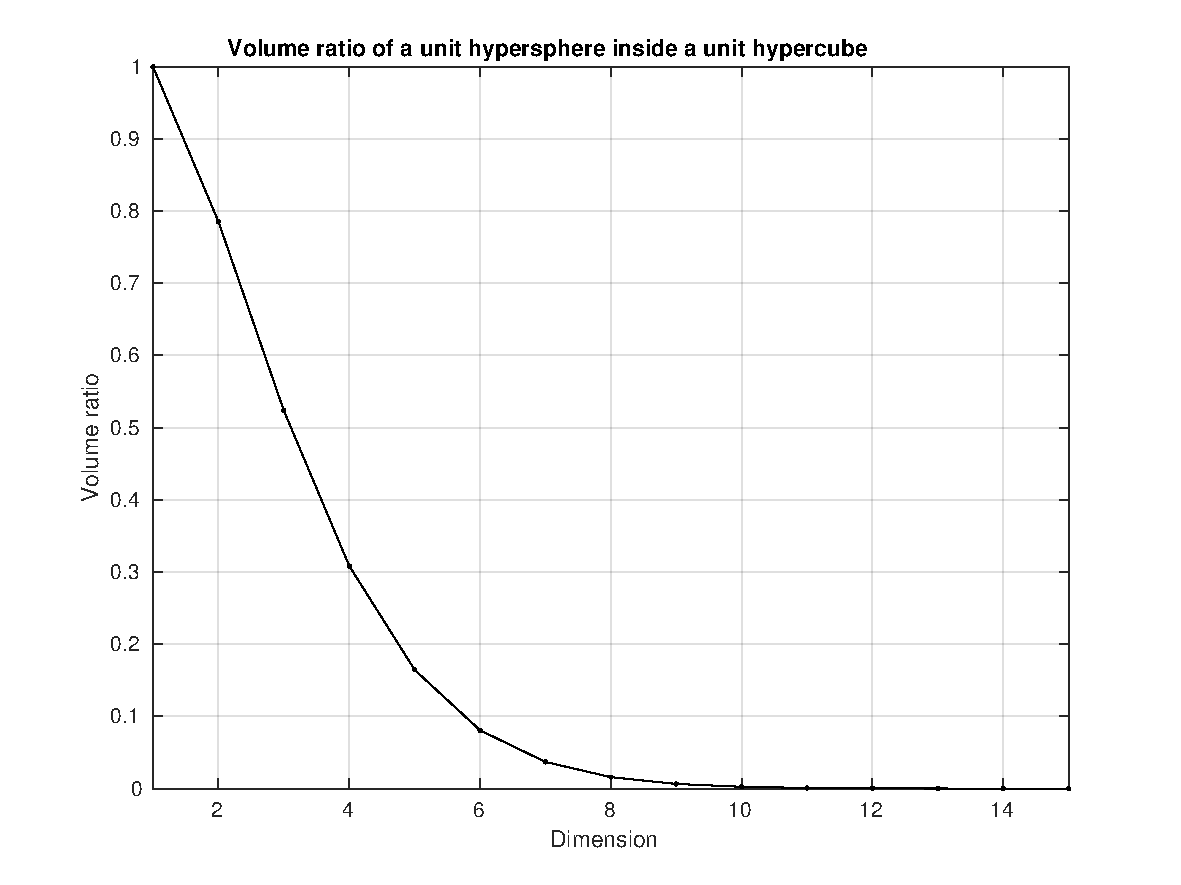
\includegraphics[scale=0.35]{hyperobjects.pdf}
	%\caption{The volume ratio of a unit hyper sphere, $2\pi^{d/2}r^d/d/\Gamma(d/2)$, inside a unit hyper cube, $(2r)^d$, as a function of dimension, $d$. This example is inspired by \citet{Laine2008}.}
	\label{hyper-objects}
\end{figure}

For a likelihood distribution over a sparse high dimensional space, the majority of the space will be extraordinarily empty - i.e. with very low probability. Considering probability is a value between 1 and 0, that means a lot of parameter space will have a likelihood very close to 0. Given this circumstance it is essential to be able to accurately compute and compare extremely small probability values. The risk of improper evaluation and comparison is erraneious steps in algorithms and a divergence from the posterior the algorithm is supposed to be sampling. In short your solution will be wrong. \par

\indent How to overcome this issue? The solution is to compute the natural logarithm of the likelihood. Figure \ref{nat-log} shows taking the natural logarithm of probability values. The result is very small probability values become very large negative numbers.

\begin{figure}[H]
	\centering
	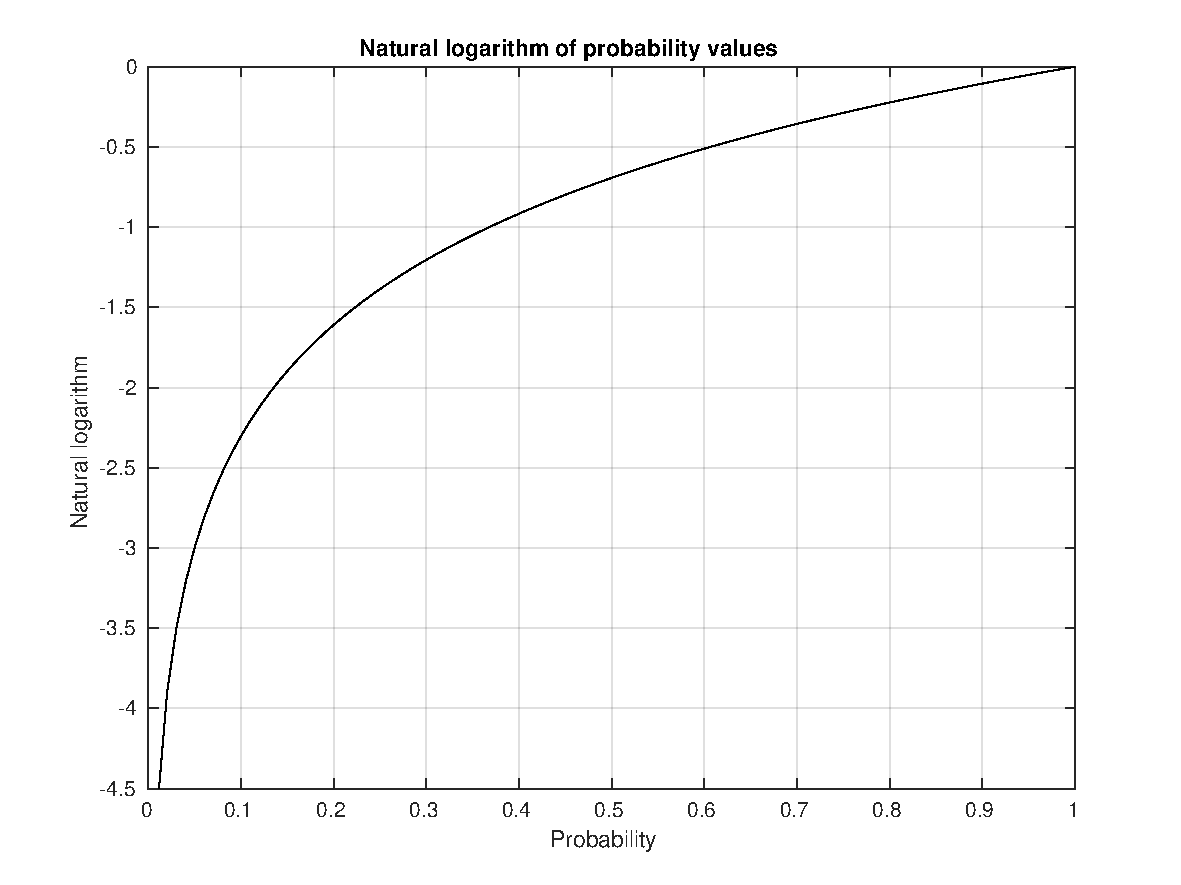
\includegraphics[scale=0.35]{nat-log.pdf}
	%\caption{The natural logarithm of probability values}
	\label{nat-log}
\end{figure}

These very large negative numbers transform a very small value, close to or crossing the limits of CPU memory, into a large number which can be easily stored. \par

\indent For a Gaussian likelihood, taking the natural logarithm of an unnormalized likelihood is in effect removing the exponential term. Consider the likelihood as in equation \ref{likelihood-2}. Repeated here
\begin{equation}
\mathcal{L}(\bm{\theta}|\bm{y}) \propto \text{exp}\bigg[-\frac{1}{2}(\bm{y}-\bm{g}(\bm{\theta}))^T(C_{\mathcal{M}}+C_{\mathcal{D}})^{-1}(\bm{y}-\bm{g}(\bm{\theta}))\bigg]
\label{repeat-likelihood-2}
\end{equation}
For $l(\bm{\theta}|\bm{y}) = \text{ln}(\mathcal{L}(\bm{\theta}|\bm{y}))$
\begin{equation}
l(\bm{\theta}|\bm{y}) \propto -\frac{1}{2}(\bm{y}-\bm{g}(\bm{\theta}))^T(C_{\mathcal{M}}+C_{\mathcal{D}})^{-1}(\bm{y}-\bm{g}(\bm{\theta}))
\label{log-likelihood}
\end{equation}
Reference to the negative log-likelihood would then mean
\begin{equation}
-l(\bm{\theta}|\bm{y}) \propto \frac{1}{2}(\bm{y}-\bm{g}(\bm{\theta}))^T(C_{\mathcal{M}}+C_{\mathcal{D}})^{-1}(\bm{y}-\bm{g}(\bm{\theta}))
\label{negative-log-likelihood}
\end{equation}

The negative log-likelihood is then a large positive number for very small probability values. Often minimization of an equation in the form of equation \ref{negative-log-likelihood} is the goal of linearized inversion schemes. Herein lies a connection between the likelihood function and linearized schemes, the result of a successful linearized inversion represents the minimum of the negative log-likelihood, $-l(\bm{\theta}|\bm{y})$. Which is also the maximum likelihood value. However our goal is generally broader. To explore the joint posterior distribution, a function of both likelihood and prior. This goal in high dimensional space necessitates Markov chain Monte Carlo (MCMC) sampling. So how does our shift to working with the natural logarithm of the likelihood impact this algorithm? \par

\indent For a MCMC algorithm with stationary distribution which is the posterior $p(\bm{\theta}|\bm{y})$, the key ingredient is evaluating the Metropolis-Hastings acceptance ratio, $\alpha$
\begin{equation}
\alpha = \frac{\mathcal{L}(\bm{\theta^*}|\bm{y})\ p(\bm{\theta^*})}{\mathcal{L}(\bm{\theta}|\bm{y})\ p(\bm{\theta})}
\label{acceptance-ratio}
\end{equation}
Where $^*$ represents a candidate move from the proposal distribution $q(\bm{\theta},.)$. As long as the proposal distribution is a symmetric distribution the ratio $q(\bm{\theta^*},\bm{\theta})/q(\bm{\theta},\bm{\theta^*})$ does not need to be computed as part of $\alpha$.\par

\indent Hence, the ratio of posterior values needs to be computed at each time step over the parameter space. The raw posterior values will be prone to numerical underflow due to the limits of CPU memory, hence the log values for the likelihood must be used in this calculation. How does the form of $\alpha$ get adjusted within a computer program to ensure stable and reliable computation?\par

\indent This shift represents a major divergence between how the theory is established in equation form, and the practical application in computer code.\par

\indent Consider we have access to the log-likelihood and log-prior. Recall the logarithm rules where $\text{ln}(xy) = \text{ln}(x)+\text{ln}(y)$ and $\text{ln}(x/y) = \text{ln}(x)-\text{ln}(y)$. Then
\begin{equation}
\alpha = \text{exp}\Big[\Big(l(\bm{\theta^*}|\bm{y})\ -\ l(\bm{\theta}|\bm{y})\Big)\ +\ \Big(\text{ln}\big(p(\bm{\theta^*})\big)\ -\ \text{ln}\big(p(\bm{\theta})\big)\Big)\Big]
\label{stable-acceptance-ratio}
\end{equation}
The resulting acceptance-ratio computed here will be equivalent to equation \ref{acceptance-ratio}, however, now the probability densities required in the computation will be restricted to large numbers, stable in their computation and comparison. The end result, a reliable MCMC algorithm.
\end{multicols}
\end{tcolorbox}
% Introduce issue which arises due to the different scale of the terms in this new Metropolis-Hastings acceptance ratio

%The shift of acceptance ratio from equation \ref{acceptance-ratio} to equation %\ref{stable-acceptance-ratio} introduces computational stability, however, a %new issue is introduced. The shift from products and ratios to addition and %subtraction means that the scales of the log-likelihoods and log-priors need %to be balanced. If one is much larger than the other then it will dominate the %calculation. This is true for calucluations of a one data set likelihood and %prior, as well as joint inversion schemes which introduce multiple individual %likelihoods into the calculation. The result has been the emergence of an ad-%hoc scaling regime for joint inversions. This directly counters the probematic %situation where the number of datapoints in the dataset leads to a %significantly different scaled log-likelihood. The standard form for joint %inversion likelihoods is given in equation XX. It can be seen that all dataset %are cobined to form a single joint log-likelihood. Two examples of scaling %schemes are
%\begin{equation}
%l_{joint} = l_1 + \frac{1}{c} l_2
%\end{equation}
%\begin{equation}
%l_{joint} = c l_1 + (1-c) l_2
%\end{equation}
%where $c$ is the scaling constant introduced. A similar scheme can be %introduced for 2+ datasets. The value of $c$ can then be set by repeated %inversion experiments which seek a known solution, the value can be taken by %what gives balanced solutions which utilise the information brought in by both %datasets.\\

%However, such a user defined weighting will be biased by our expectations in %synthetic tests. The final uncertainties may not accurately reflect the %uncertainty present in a real world problem. This may mean compromised %statistical properties the probabilitic Bayesian method guarentees to deliver.  %\\

%At this stage there is no "solution". A joint likelihood which utilises user %defined weights is currently the accepted system for joint inversion. But this %system should not be blindly accepted. Part of the scope of this thesis is %question the statistical underpinning of this form of the likelihood and probe %alternate formulations.


\section{Approximate Bayesian Computation}
\label{ApproximateBayesianComputation}

The likelihood, while underpinning a system which is formally strong and practically useful for geophysics, does suffer some weaknesses which are implicit in its construction and application. The likelihood limits the number of models (combined deterministic forward and uncertainty) which can be considered and applied as it requires a closed form expression. It relies on informal tuning for joint inversions which may compromise the strict formal statistical properties which the Bayesian method guarantees to deliver. The likelihood also mixes and dilutes the available information about the data fit and model into a single metric. While necessary in the likelihood framework, this may not be the best way to drive an inversion scheme. Other disciplines have found Approximate Bayesian Computation offers an alternative to traditional likelihood machinery which can utilize more of what is known about the structure, physics and nature of the parameter inference problems at hand \citep{Tavare1997,Ratmann2009,vrugt2013toward}. It opens inference to a broader range of models and likewise offers formal statistical guarantees \citep{Sunnaker2013}.\par

Likelihood-free methods for Bayesian inference have been developed in response to parameter estimation problems where it is not possible to formulate or justify a closed form likelihood function (e.g. \citet{Tavare1997,Fu1997,Weiss1998a,Pritchard1999a,Beaumont2002,Marjoram2003}). Instead, likelihood-free methods target the same posterior distribution without evaluating a likelihood function. The algorithms and methods of likelihood-free Bayesian inference have been termed \textit{Approximate Bayesian Computation} (ABC). ABC simply requires the ability to simulate data given model parameters. Problems ripe for attack by ABC are common in science due to the breadth of models which have been developed to describe natural systems. It is frequently the case that the uncertainty associated with the data can be simulated rapidly but explicit formulas for probability distributions are difficult to formulate, expensive to evaluate, impossible to justify, or do not exist. Hence, traditional likelihood machinery becomes infeasible. ABC is a means to overcome these issues, it is backed by a sound theoretical underpinning and is subject to a rapidly expanding set of literature \citep{Ratmann2009,Blum2010,vrugt2013toward,Sunnaker2013,Blum2013,Sadegh2014,Pudlo2015,meeds2015hamiltonian,Lintusaari2016,gutmann2016bayesian,sisson2016handbook,Li2017}. \par

The premise of ABC begins with the notion that a set of model parameters, $\bm{\theta}$, is a sample from the posterior if the observed data, $\bm{y}$, and a simulated dataset, $\bm{y^*}$, are equal. Algorithm \ref{basicalg} generates i.i.d samples from the posterior $p(\bm{\theta}|\bm{y})$ (cf. \citet{Marjoram2003}).

\begin{algorithm}[H]
	\caption{ }
	\begin{algorithmic}
		\State 1. Generate $\bm{\theta^*}$ as a random sample from $p(\bm{\theta})$		
		\State 2. Simulate $\bm{y^*}$ from the forward operator $\bm{g_s}(\bm{\theta^*})$		
		\State 3. Accept $\bm{\theta^*}$ as a posterior sample if $\bm{y^*} = \bm{y}$		
		\State 4. Repeat
	\end{algorithmic}
	\label{basicalg}
\end{algorithm}

The operator $\bm{g_s}$ in Algorithm \ref{basicalg}, and all of likelihood-free inference, differs from the forward operators traditionally defined in geophysics. Forward operators in geophysics are \textit{deterministic}. That is, for a given set of model parameters, $\bm{\theta}$, the output of the forward operator $\bm{g}(\bm{\theta})$ will always be the same. The uncertainty in both data and model, are then later built into the construction of a likelihood function. The ABC forward operator which simulates data, $\bm{g_s}$, is \textit{stochastic}. That is, the uncertainty from both data and modelization is built into the simulation process. As a result of this modification, algorithm \ref{basicalg} does not require the formulation or evaluation of a likelihood function. The ABC forward operator $\bm{g_s}$ allows a practitioner to build in whatever uncertainty is justified for the scientific problem at hand. \par

Algorithm \ref{basicalg} is acceptable for basic problems where the datasets $\bm{y}$ and $\bm{y^*}$ is a discrete probability function, e.g. integers \citep{Tavare1997,Fu1997}. However, for large and continuous datasets the probability of generating a sample where the acceptance criteria, $\bm{y^*} = \bm{y}$, is met diminishes to levels unacceptable for parameter inference. ABC relaxes the problematic requirement of equality by accepting samples when the distance between $\bm{y^*}$ and $\bm{y}$, $\text{d}(\bm{y},\bm{y^*})$, is less than a tolerance value $\epsilon$ \citep{Weiss1998a}. This method, algorithm \ref{ABCfulldatatolerance}, does not target our true posterior of interest, but instead, the ABC posterior $p(\bm{\theta}|\text{d}(\bm{y},\bm{y^*})\leq\epsilon)$ which approximates the true posterior. 

\begin{algorithm}[H]
	\caption{ }
	\begin{algorithmic}
		\State 1. Generate $\bm{\theta^*}$ as a random sample from $p(\bm{\theta})$		
		\State 2. Simulate $\bm{y}$ from the forward operator $\bm{g_s}(\bm{\theta^*})$		
		\State 3. Accept $\bm{\theta^*}$ as a posterior sample if $\text{d}(\bm{y},\bm{y^*})\leq\epsilon$		
		\State 4. Repeat
	\end{algorithmic}
	\label{ABCfulldatatolerance}
\end{algorithm}

Algorithm \ref{ABCfulldatatolerance} requires a user specified metric, $\text{d}$, which defines the distance between datasets. Common choices are the absolute-value norm, Euclidean distance and Mahalanobis distance. Likewise, the value for the tolerance $\epsilon$ must be user specified. As $\epsilon \rightarrow \infty$, the sampled target distribution of algorithm \ref{ABCfulldatatolerance} $p(\bm{\theta}|\text{d}(\bm{y},\bm{y^*})\leq\epsilon) \rightarrow p(\bm{\theta})$.  Algorithm \ref{ABCfulldatatolerance} simply recovers the prior distribution. However, as $\epsilon \rightarrow 0$ the sampled distribution $p(\bm{\theta}|\text{d}(\bm{y},\bm{y^*})\leq\epsilon) \rightarrow p(\bm{\theta}|\bm{y})$. The exact posterior is recovered. Encoded in the value of $\epsilon$ is a trade-off between acceptance rate and accuracy. As $\epsilon$ increases so does the efficiency of the sampler, but the accuracy of the recovered distribution is increasingly eroded \citep{Sisson2010a}. Conversely, as $\epsilon$ decreases the accuracy of the recovered distribution converges to the true posterior, but the acceptance rate approaches computationally infeasible levels. This trade-off for computational efficiency at the cost of accuracy is where ABC derives the name \textit{Approximate} Bayesian Computation, as the samplers recover a distribution which approximates the true posterior.\par

% Write about summary statistics
Rejection sampler inference in the form of algorithm \ref{ABCfulldatatolerance} can run into efficiency problems as the dimensionality (size) of the datasets grow. In this case the probability of sampling $\text{d}(\bm{y},\bm{y^*})\leq\epsilon$ diminishes as the size of the dataset grows. Since first application \citep{Tavare1997} likelihood-free methods have adopted the use of low-dimensional summary statistics about the data in the evaluation of distance, $\text{d}$. A metric over a vector of summary statistics is evaluated, $\text{d}(\bm{S}(\bm{y}),\bm{S}(\bm{y^*}))$. This leads to the most common form of an ABC rejection sampling scheme of algorithm \ref{ABCrejectionsampler} \citep{Pritchard1999a}. This rejection sampler generates i.i.d samples from the distribution $p(\bm{\theta}|\text{d}(\bm{S}(\bm{y}),\bm{S}(\bm{y^*}))\leq\epsilon)$.

\begin{algorithm}[H]
	\caption{ }
	\begin{algorithmic}
		\State 1. Generate $\bm{\theta^*}$ as a random sample from $p(\bm{\theta})$		
		\State 2. Simulate $\bm{y}$ from the forward operator $\bm{g_s}(\bm{\theta^*})$		
		\State 3. Compute summary statistics $\bm{S}(\bm{y})$ and $\bm{S}(\bm{y^*})$		
		\State 4. Accept $\bm{\theta^*}$ as a posterior sample if $\text{d}(\bm{S}(\bm{y}),\bm{S}(\bm{y^*}))\leq\epsilon$		
		\State 5. Repeat
	\end{algorithmic}
	\label{ABCrejectionsampler}
\end{algorithm}

In the first application of likelihood-free inference, \citet{Tavare1997} replace the full sequences of DNA with the number of sites which differ between DNA samples. The idea being that as long as the statistics used are \textit{sufficient} there is no information loss for parameter inference. As a result of sufficiency the posterior computed with statistics will be equivalent to the the posterior computed by the full dataset, i.e $p(\bm{\theta}|\bm{S}(\bm{y})) = p(\bm{\theta}|\bm{y})$. It is often the case that no truly sufficient statistics exist for problems of scientific interest. Instead practitioners settle for a reasonably sufficient low-dimensional set of summary statistics. This lack of sufficiency introduces a second bias, tolerance being the first, into the ABC-posterior $p(\bm{\theta}|\text{d}(\bm{S}(\bm{y}),\bm{S}(\bm{y^*}))\leq\epsilon)$ due to the information lost by summarizing the full data set. It is, however, thanks to summary statistics that likelihood-free inference owes it's origin and can proceed. Summary statistics have allowed parameter inference to be applied to problems as challenging as noisy near-chaotic ecology populations \citep{Wood2010} and have been shown to offer superior power to diagnose model insufficiency \citep{Ratmann2009,vrugt2013toward}.\par

% talk about MCMC-ABC
Seminal developments in ABC have considered algorithms and equations in the form which have been introduced so far \citep{Fu1997,Pritchard1999a,Beaumont2002,Marjoram2003}. However, ABC can be cast in another mathematical light which enables straight forward implementation into sampling routines such as MCMC. The stochastic forward simulations from ABC, $\bm{y^*}$, are viewed as an auxiliary parameter which is introduced into the posterior to facilitate computation \citep{Sisson2010a}. This process changes the computed posterior from the traditional $p(\bm{\theta}|\bm{y}) \propto p(\bm{y}|\bm{\theta})p(\bm{\theta})$ to the ABC posterior:

\begin{equation}
p_{ABC}(\bm{\theta},\bm{y^*}|\bm{y}) \propto p(\bm{y}|\bm{y^*},\bm{\theta}) p(\bm{y^*}|\bm{\theta}) p(\bm{\theta})
\label{eqABCposterior}
\end{equation}

where $\bm{y^*}$ is viewed as a realization from the density $p(\bm{y^*}|\bm{\theta})$. $p(\bm{y}|\bm{y^*},\bm{\theta})$ is introduced to serve the same role as the accept/reject step in Algorithms \ref{ABCfulldatatolerance} and \ref{ABCrejectionsampler}. $p(\bm{y}|\bm{y^*},\bm{\theta})$ is chosen to weight the posterior with high values when the observed and simulated datasets are close. However, the form of equation \ref{eqABCposterior} allows the mathematics of kernel densities to be introduced into $p(\bm{y}|\bm{y^*},\bm{\theta})$ such that \citep{Sisson2010a}:
\begin{equation}
p(\bm{y}|\bm{y^*},\bm{\theta}) = \frac{1}{\epsilon} K \Big(\frac{\text{d}(\bm{y},\bm{y^*})}{\epsilon}\Big)
\label{generic-weighting-kernel}
\end{equation}
Where $K$ is some standard kernel, and the tolerance $\epsilon$ serves as the kernel bandwidth. \par

Thinking of equation \ref{eqABCposterior} in algorithm form still allows a straightforward understanding.
\begin{algorithm}[H]
	\caption{ }
	\begin{algorithmic}
		\State 1. Generate $\bm{\theta^*}$ as a random sample from $p(\bm{\theta})$		
		\State 2. Simulate $\bm{y}$ from the forward operator $\bm{g_s}(\bm{\theta^*})$		
		\State 3. The distance between simulated and observed datasets is evaluated		
		\State 4. The parameter set is accepted with probability equal to $p(\bm{y}|\bm{y^*},\bm{\theta})$	
		\State 5. Repeat
	\end{algorithmic}
	\label{algorithm-form-equation}
\end{algorithm}

While equation \ref{eqABCposterior} targets the joint posterior density of simulations and model parameters, marginalization to our posterior of interest, $p_{abc}(\bm{\theta}|\bm{y})$, is done numerically by discarding the simulations recovering:
\begin{equation}
p_{ABC}(\bm{\theta}|\bm{y}) \propto p(\bm{\theta}) \int_{\bm{y^*}} p(\bm{y}|\bm{y^*},\bm{\theta}) p(\bm{y^*}|\bm{\theta})\ \text{d}\bm{y^*}
\label{eqABCtargetPosterior}
\end{equation}\par

Equation \ref{eqABCtargetPosterior} can be adjusted to rely on summary statistics. The density $p(\bm{S}(\bm{y^*})|\bm{\theta})$ is introduced as the density implied from taking summary statistics about $p(\bm{y^*}|\bm{\theta})$ and $p(\bm{S}(\bm{y})|\bm{S}(\bm{y^*}),\bm{\theta})$ is a kernel over the distance between summary statistics. Our approximate Bayesian posterior distribution becomes:
\begin{equation}
p_{ABC}(\bm{\theta}|\bm{S}(\bm{y})) \propto p(\bm{\theta}) \int_{\bm{S}(\bm{y^*})} p(\bm{S}(\bm{y})|\bm{S}(\bm{y^*}),\bm{\theta})\  p(\bm{S}(\bm{y^*})|\bm{\theta})\ \text{d}\bm{S}(\bm{y^*})
\label{summary-stat-abc-posterior}
\end{equation}

\citet{Marjoram2003} first demonstrated a Markov chain Monte Carlo (MCMC) scheme to sample the ABC posterior distribution. A simple MCMC algorithm with a Metropolis-Hastings (MH) acceptance probability is demonstrated in algorithm \ref{ABC-MCMC}. The M-H acceptance probability $\alpha$ to recover the ABC posterior is:
\begin{equation}
\alpha_{ABC} = \frac{p(\bm{S}(\bm{y})|\bm{S}(\bm{y^*}),\bm{\theta})\ p(\bm{\theta^*})\ q(\bm{\theta^*},\bm{\theta_{t-1}})} {p(\bm{S}(\bm{y})|\bm{S}(\bm{y_{t-1}}),\bm{\theta})\ p(\bm{\theta_{t-1}})\ q(\bm{\theta_{t-1}},\bm{\theta^*})}
\label{M-H-acce}
\end{equation}
Where $\bm{t}$ denotes the time step in the chain, and $\bm{\theta^*}$ is used to represent a candidate move from the proposal distribution $q(\bm{\theta_{t-1}},\cdot)$.

\begin{algorithm}[H]
	\caption{ }
	\begin{algorithmic}
		\State 1. Start from an initial state $\bm{\theta^0}$ and select a proposal distribution $q(\cdot,\cdot)$
		\State 2. At each step where the current state is $\bm{\theta_{t-1}}$, propose a candidate 	move $\bm{\theta^*}$ from the distribution $q(\bm{\theta_{t-1}},\cdot)$		
		\State 3. If the candidate state is better than the previous state, $\alpha_{ABC} > 1$, then the candidate state is accepted unconditionally meaning $\bm{\theta_t} = \bm{\theta^*}$
		\State 4. If the candidate move is not better in the above sense, then $\bm{\theta^*}$ is accepted with probability equal to $\alpha_{ABC}$		
		\State 5. If the candidate move is not accepted, then the chain remains in its current state, meaning $\bm{\theta_{t}} = \bm{\theta_{t-1}}$		
		\State 6. Repeat the simulation steps 2-5 until enough values have been generated
	\end{algorithmic}
	\label{ABC-MCMC}
\end{algorithm}

% Give a general history and propose a goal and oulook for the analysis
ABC originated from applied problems where a likelihood was not available. As we saw in the last section, and expanded upon in \hyperref[tf2]{technical figure 2}, geophysics has been able to leverage likelihoods, for example, in the form of equations \ref{likelihood-1} and \ref{likelihood-2}. This access to a likelihood is the direct result of the assumptions about the statistical properties of the measurement and modelization uncertainty. However, under more complex models for uncertainty, an analytical formula for the likelihood may not be accessible. This is where ABC algorithms have traditionally been able to step in, bypassing using a likelihood, and in the process opening parameter inference a range of more complex models. \par

%Our hope is that ABC can offer improvements over several limiting aspects of traditional likelihood based Bayesian inference. These improvements may be focused around several aspects. One is computing a joint likelihood in a balanced and statistically uncompromisable manner. Another is making inversion schemes more diagnostic. At each step in an algorithm we can leverage the full dataset to decide what is the next appropriate move. Truly realistic uncertainty can be introduced, free from simplifications required for formulating the analytical PDFs or needed for computational simplicity. Inversion schemes can potentially balance the trade off between excessively wasteful Monte Carlo methods, requiring millions of forward simulations and the extraordinarily stringent budget of linearized methods. Also, the freedom ABC allows may facilitate introducing some components of existing geophysical knowledge into the the inversion scheme where appropriate. This may be gradients of relevant functions for suggesting model updates or sensitivity kernels for the evaluation of fitness. In short, the freedom of ABC may allow us to open our eyes to alternatives which diverge from the current paradigm of joint inversion schemes. \par

The main postulate of this thesis is that ABC can offer improvements over some limiting aspects of traditional likelihood based Bayesian inference. This improvement may be focused in several different areas. ABC does not make the requirement for Gaussian distributed uncertainty. This may allow, for example, realistic measurement and modelization uncertainties to be incorporated into the inversion scheme. ABC can uniquely investigate the adequacy of the model in absolute terms against the data, as opposed to relative to the performance of other models (ABC$\mu$ of \citet{Ratmann2009}). This allows fundamental deficiencies in the model to be exposed. While the closed form expression for the likelihood requires the mixing and dilution of information into a single metric, this is not required of ABC. ABC may be capable of considering the full scope of information available within a simulated dataset to drive a diagnostic inversion. In short, the freedom of ABC provides an alternative to the current paradigm of inversion schemes. In the same way approximate numerical methods allow us to tackle a greater number of problems than otherwise possible with analytical solutions. \par

Many of the above possibilities are outside the scope of an 9 month Masters' project. However these will serve as guiding aims and potential for future exploration. My goal here is to simply demonstrate some advantage of a geophysical ABC scheme, which will motivate future investigation.

% Other chapters in here
\chapter{ABC}

This chapter will outline a series of illustrative ABC examples. These will serve to demonstrate core concepts touched on in the introduction, demonstrate ABC can sample from complex distributions, and develop the boutique code base which form the foundations of this project. The code for the examples in this section can be found at \url{https://github.com/tomconnell/dram}.\\

\section{Toy problem 1: 1D Gaussian}
As a simple first example consider we have observed $n = 100$ realizations from the Gaussian model $\bm{g_s}(\bm{\theta}) = \frac{1}{\sqrt{2\pi\sigma^2}}\ \text{exp}\Big[\frac{-\mu^2}{2\sigma^2}\Big]$. Our unknown model parameters are $\bm{\theta} = [\mu,\sigma]$. Given we have access to simulation from this model it is possible to leverage ABC algorithms to estimate these unknown model parameters. A synthetic dataset for this problem is created with $\mu = 5$ and $\sigma = 2$. The summary statistics sample mean, $\bar{\mu}$, and sample standard deviation, $\bar{\sigma}$, are used. These provide sufficient statistics with a 1:1 correspondance to the unknown parameters. Figure \ref{toy1-fig1} plots the ABC posterior obtained from using algorithm \ref{ABCrejectionsampler}, the traditional form of an ABC rejection sampler, compared to the analytical likelihood. The metric over summary statistics is evaluated marginally and hence takes the form $\rho = |S_1(\bm{y^*}) - S_1(\bm{y})| +| S_2(\bm{y^*}) - S_2(\bm{y})|$. A uniform prior is used to give equal probability to a bounded area, $p(\mu) = \mathcal{U}(0,10)$ and $p(\sigma) = \mathcal{U}(0,10)$. 
Figure \ref{toy1-fig2} explores the impact of varying the tolerance for this problem.\\

\begin{figure}[H]
	\centering
	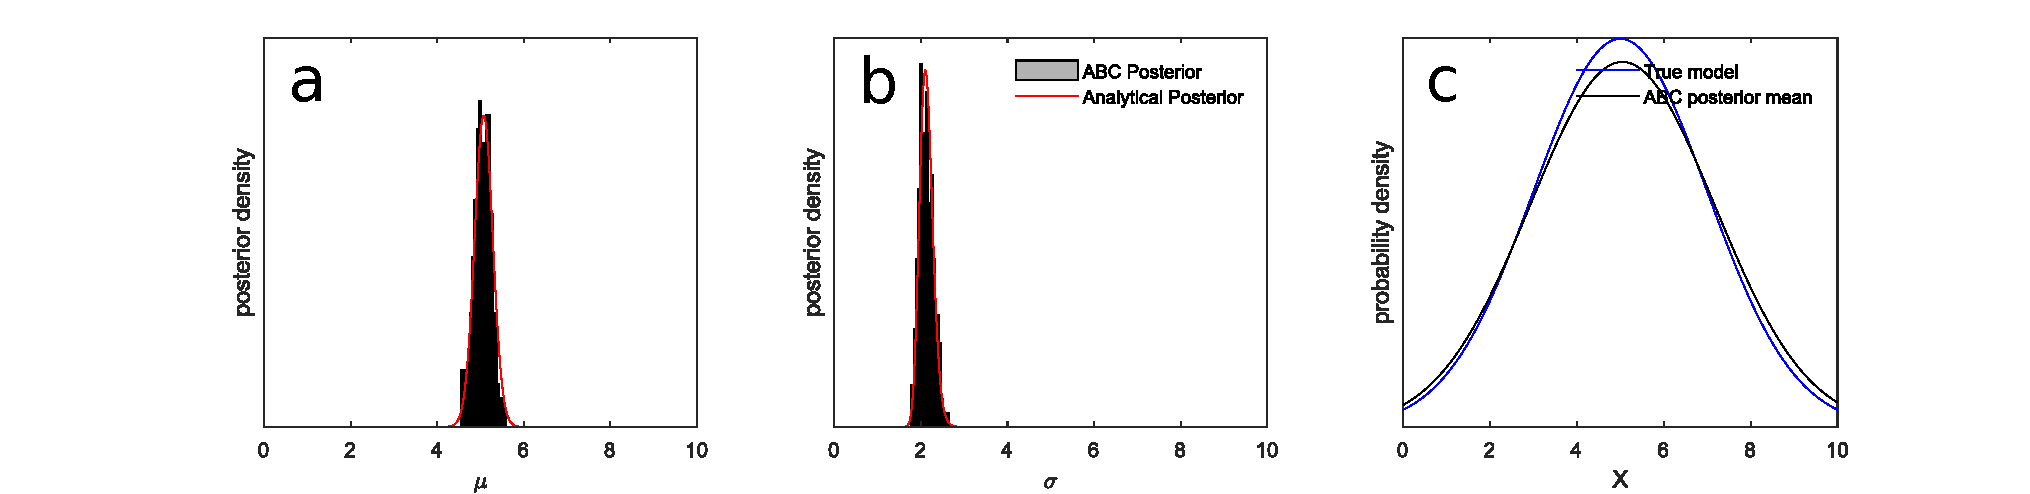
\includegraphics[scale=0.45]{toy1-fig1.pdf}
	\caption{Posterior comparison between ABC and traditional likelihood inference for estimating the parameters, $\bm{\theta} = [\mu,\sigma]$, to a Gaussian model given $n = 100$ observations, $\bm{y}$. The ABC algorithm, algorithm \ref{ABCrejectionsampler}, uses 1 million repititions and a tolerance $\epsilon = 0.1$. The likelihood takes the form $\mathcal{L}(\bm{\theta}|\bm{Y}) = (2\pi\sigma^2)^{-n/2}\ \text{exp}\big[-\frac{1}{2\sigma^2}\sum_{i = 1}^{n}(y_i-\mu)^2\big]$. (a) Marginal posterior compared to marginal ABC posterior for unknown parameter $\mu$. (b) same as (a) but for unknown parameter $\sigma$. (c) Mean ABC posterior model compared to true model.}
	\label{toy1-fig1}
\end{figure}

\begin{figure}[H]
	\centering
	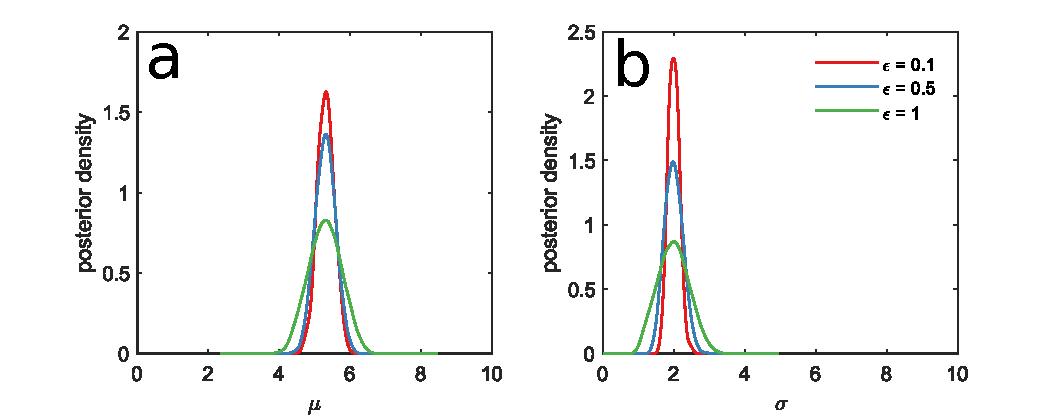
\includegraphics[scale=0.6]{toy1-fig2.pdf}
	\caption{The effect of varying the tolerance $\epsilon$ when estimating $\bm{\theta} = [\mu,\sigma]$ to a Gaussian model given given $n = 100$ observations, $\bm{y}$. Three tolerances are considered, $\epsilon = 0.1$, $\epsilon = 1$, $\epsilon = 5$. (a) Marginal ABC posterior for unknown parameter $\mu$. The true value is $\mu = 5$ (b) same as (a) but for unknown parameter $\sigma$. The true value is $\sigma = 2$}.
	\label{toy1-fig2}
\end{figure}

Figure \ref{toy1-fig1} demonstrates that with sufficient statistics and a low tolerance ABC can accurately resolve the posterior using only the ability to simulate data. However, as figure \ref{toy1-fig2} demonstrates, high tolerances significantly erode posterior accuracy and uncertainty is significantly over-estimated. However, it is true that increasing the tolerance increases the acceptance rate and hence relaxes computational resources. In this case the acceptance rate with $\epsilon = 0.1$ was $0.021\%$, while the acceptance rate with $\epsilon = 1$ was $2.023\%$. Under a model which is expensive to simulate from walking the tightrope between accuracy and efficiency becomes important and needs to be carefully examined. In spite of shortcomings, the strengths of the ABC rejection sampler has led to significant scientific experiments \citep{Fu1997,Weiss1998a,Pritchard1999a}.

\section{Toy problem 2: Linear regression}
\label{sec-lin-reg}

As a second example consider we have observed some data, $\bm{y}$, from the linear model $\bm{g}(\bm{\theta}) = m\bm{x} + b$ and there is some stochasticity in the measurement process such that $\bm{g_s}(\bm{\theta}) = \bm{g}(\bm{\theta}) + \mathcal{N}(0,\sigma^2)$. Our unknown parameters are $\bm{\theta} = [m,b]$, while $\sigma$ is known. In this case it is deemed that computational resources are limitied and MCMC, which uses local transitions, will be needed to improve acceptance rates. MCMC will also be needed when the search spaces are high dimensional, many unknown parameters, and the posterior is a long way from the prior. For this case we can call upon ABC-MCMC in the form of algorithm \ref{ABC-MCMC}. \\

Algorithm \ref{ABC-MCMC} samples the ABC posterior, equation \ref{summary-stat-abc-posterior}. The algorithm relies on evaluating the M-H acceptance probability, equation \ref{M-H-acce}. In our implementations Gaussian transition kernels, $q(.,.)$, are strictly used. As such the transition kernels cancel out in equation \ref{M-H-acce}. That leaves the prior and the weighting kernel to be evalutated at each time step in the Markov chain. The weighting kernel takes the form of equation \ref{generic-weighting-kernel}. In this case a uniform weighting kernel, $K_U$, is implemented. The interpretation of $K_U$ is the same as the accept/reject step in the rejection sampler: 
\begin{equation}
	K_U = 
	\begin{cases}
		1 & \text{if}\ 	\frac{|(S_i(\bm{y^*}) - S_i(\bm{y}))|}				{\epsilon_i} \leq 1\\
		0 & \text{if}\ \frac{|(S_i(\bm{y^*}) - S_i(\bm{y}))|}				{\epsilon_i} > 1
	\end{cases}
\end{equation}
$K_U$ hence forms an indicator function $\mathbbm{1}$ which is equal to $1$ when the distance between statistics, which are fit marginally, is less than the tolerance. Given, $\bm{S} = \{S_1,\dots,S_O\}$, the weighting kernel takes the form:
\begin{equation}
	p(\bm{S}(\bm{y})|\bm{S}(\bm{y^*}),\bm{\theta}) = \prod_{i = 1}^{O} K_U\Big(\frac{\rho(S_i(\bm{y}),S_i(\bm{y^*})}{\epsilon_i}\Big)
	\label{weight-kernel}
\end{equation}
\noindent
As with the 1D Gaussian example it would be possible to take summaries which have a 1:1 correspondance to the unknown parameters. For a given simulation, a linear model could be fit to the simulated data and the slope and intercept used as summaries. However, to demonstrate that this is not necessary, we take inspiration from \citet{vrugt2013toward} and use mean, $\mu$, and standard deviation, $\sigma$, as summary statistics. The slope is restricted to a positive value to make these statistics sufficient. \\

Figure \ref{linear-regression} shows ABC-MCMC applied to the linear regression problem. \\

This example truly highlights how ABC shifts away from many traditional Bayesian and frequentist techniques which rely computing data residuals in the form $\sum (\bm{g}(\bm{\theta})-\bm{y})^2$. This residual is computed in the analytical linear regression likelihood and is at the heart of all likelihood functions which are applied in geophysics, equation \ref{likelihood-1} and equation \ref{likelihood-2}. Instead, ABC opts for informal measures of 'goodness-of-fit' and rely on user-varied tolerances, which guarentee posteriors close-to the true posterior, save for a small degree of bias. The result of a tolerance $> 0$ and summary statistics which do not always measure fitness as tightly as a data residual. However the gain is in diagnostic power. The data residual takes all the information in the data set and mixes it into a single number, the residual value. However, the form of ABC allows for the state of the algorithm at any one stage to be evaluated and fitting statistics marginally means different rules can be set for different statistics depending on what they mean to the inversion. Understanding how statistics change through an inversion, the nature in which they diverge, and the degree to which they spread around the observed value has taught researches in other disciplines a great deal about the nature of their models and the systems in which they study. That same central idea should be transferrable to geophysical parameter estimation problems and may offer room for more diagnostic inversion schemes, one with a greater deal of user control and greated deal of interprebable meaning. \\

In the next section we continue to introduce algorithmic considerations into ABC as we build toward a geophysically relevant parameter estimation system. \\

\begin{figure}[H]
	\centering
	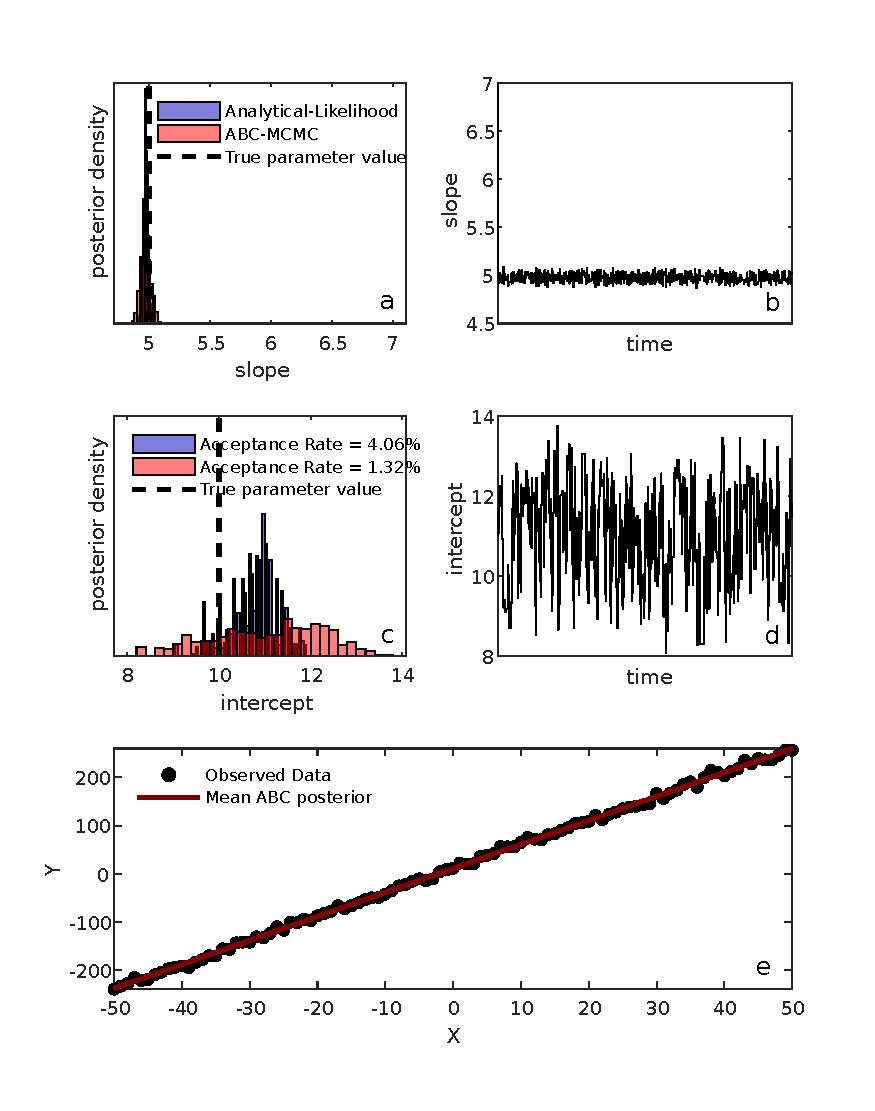
\includegraphics[scale=1.1]{linear-regression-example.pdf}
	\caption{Linear regression with ABC. The ABC posterior is also compared to traditional likelihood machinary. MCMC is used for both posteriors. The tolerance is $\bm{\epsilon} = [2,2]$ and the transition kernel is $q = \mathcal{N}([0,0],I)$. The Markov chain length is $20\ 000$. (a) The marginal ABC posterior and marginal analytical posterior compared for unknown parameter $m$. (b) Plot of Markov chain through time for $m$. (c) Same as (a) except for unknown parameter $b$. (d) Same as (b) except for unknown parameter $b$. (e) Comparison of the mean ABC posterior model and the observed data generated with $m = 5$, $b = 10$ and $\sigma = 5$.}
	\label{linear-regression}
\end{figure}

\section{Toy problem 3: Bivariate Gaussian}
% Introduce the problem
As a third example consider we $n = 100$ observations from a bivariate Gaussian distribution $\mathcal{N}(\bm{\mu},\bm{\Sigma})$ with $\bm{\mu} = \begin{bmatrix}
\mu_X\ \mu_Y
\end{bmatrix}^T$ and $\bm{\Sigma} = \begin{bmatrix}
\sigma^2_X & \rho\sigma_X\sigma_Y\\
\rho\sigma_X\sigma_Y & \sigma^2_Y
\end{bmatrix} $ where both $\bm{\mu}$ and $\bm{\sigma}$ are unknown, hence $\bm{\theta} = [\bm{\mu},\bm{\Sigma}]$. Figure \ref{init-qualms}(a) shows the observed data and the underlying causitive distribution. This example has 5 unknown parameters in total and as such we can appeal to ABC-MCMC for efficient sampling. The weighting kernel takes the same for as equation \ref{weight-kernel} and summaries with a 1:1 correspondance to the unknown parameters are used, the marginal sample means and standard deviations, as well as sample covariance. The prior distribution, $p(\bm{\theta}) = \mathcal{U}(0,10)$, is used to provide equal probability to a bounded area for all unknowns beside correlation, $\rho$, which bounded as $p(\rho) = \mathcal{U}(-1,1)$. Figure \ref{init-qualms}(b) shows the results of the first 10000 time steps from an ABC-MCMC. It can be seen that the algorithm is stationary for the first 3000 repititions.\\

%% Figure a of the observed data and figure b of the stuck chain
\begin{figure}[H]
	\centering
	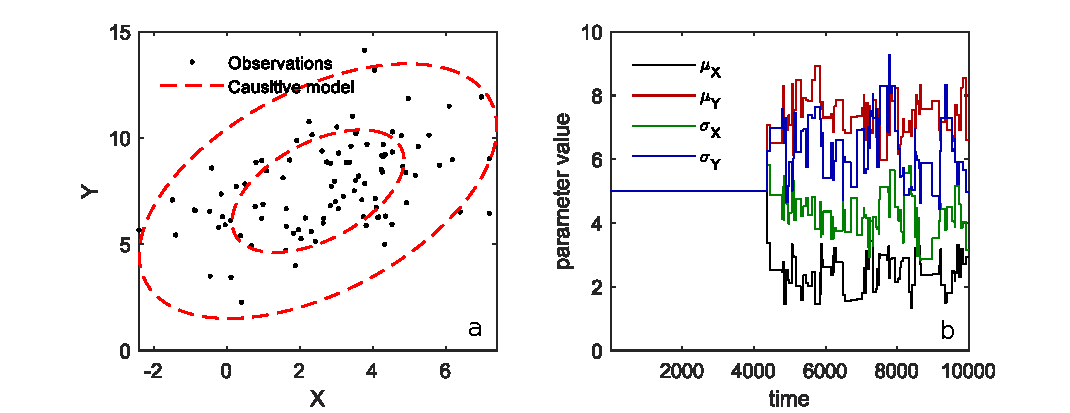
\includegraphics[scale=0.75]{init-problems.pdf}
	\caption{}
	\label{init-qualms}
\end{figure}

%Figure of the chain becoming stuck at the beggining

While ABC-MCMC and the uniform weighting kernel $K_U$ offered invariably improved acceptance rates compared to a rejection scheme in Figure \ref{linear-regression}, it is not without faults. Firstly, it can suffer from an initialisation problem, as highlighted in figure \ref{init-qualms}(b). This is discussed extensively by \citep{Sisson2010a} as they search for solutions which can overcome the initialisation problem, while still using $K_U$. Compounding this, the acceptance rate can rapidly decline past a certain threshold as tolerance is decreased. That is a syptom of the same problem as with initialisation. Each move is either flat out rejected or is determined to be part of the posterior. This makes it prone to becoming stuck when in the tails of a distribution. This is especially problematic in high-dimensional search spaces where the posterior density is an extraordinarily small volume within the parameter space. Ideally, if in a poor spot, the algorithm should be able to make local transitions toward an area of high probability density. However, this adjustment will invove abandoning the uniform kernel. What is needed is a weighting kernel which offers infinite support. That is, the weight dimishes with distance, however it never reaches zero. Fortunately many functions have the required properties. In this text we favour a  weighting kernel based on the Gaussian distribution, $K_G$. The Gaussian distribution is able to be evaluated in a computationally stable way, even as the weighting terms reach extraordinarily small values. See Appendix B for an outline of the stable computational evaluation of the weighting kernel.\\

\begin{equation}
K_G(u) = 
\end{equation}

\begin{figure}[H]
	\centering
	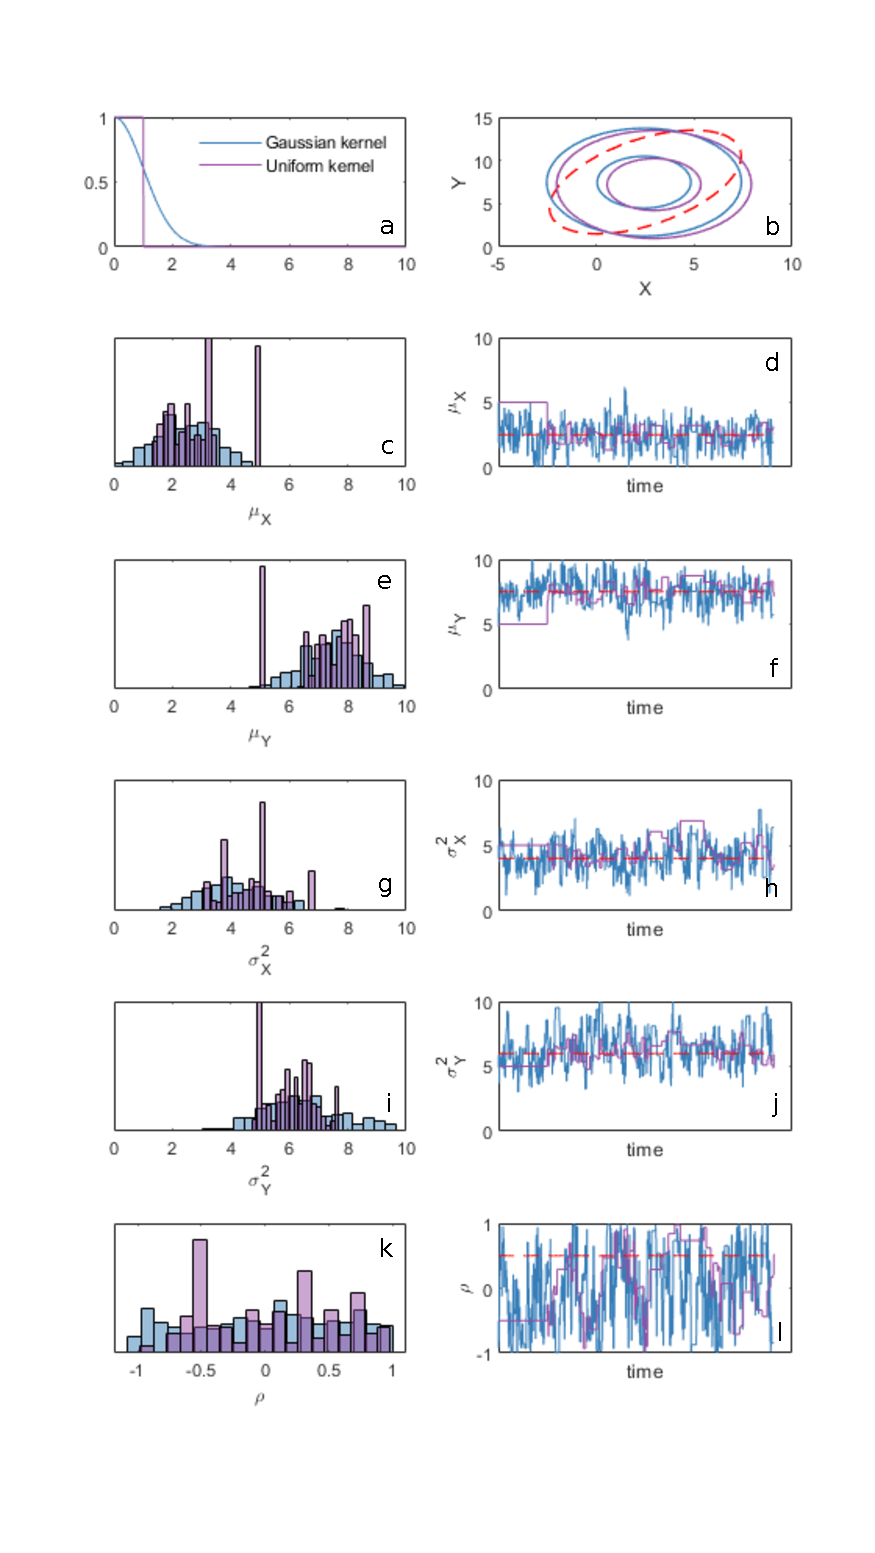
\includegraphics[scale=0.8]{BG7500.pdf}
	\caption{}
\end{figure}

\begin{figure}[H]
	\centering
	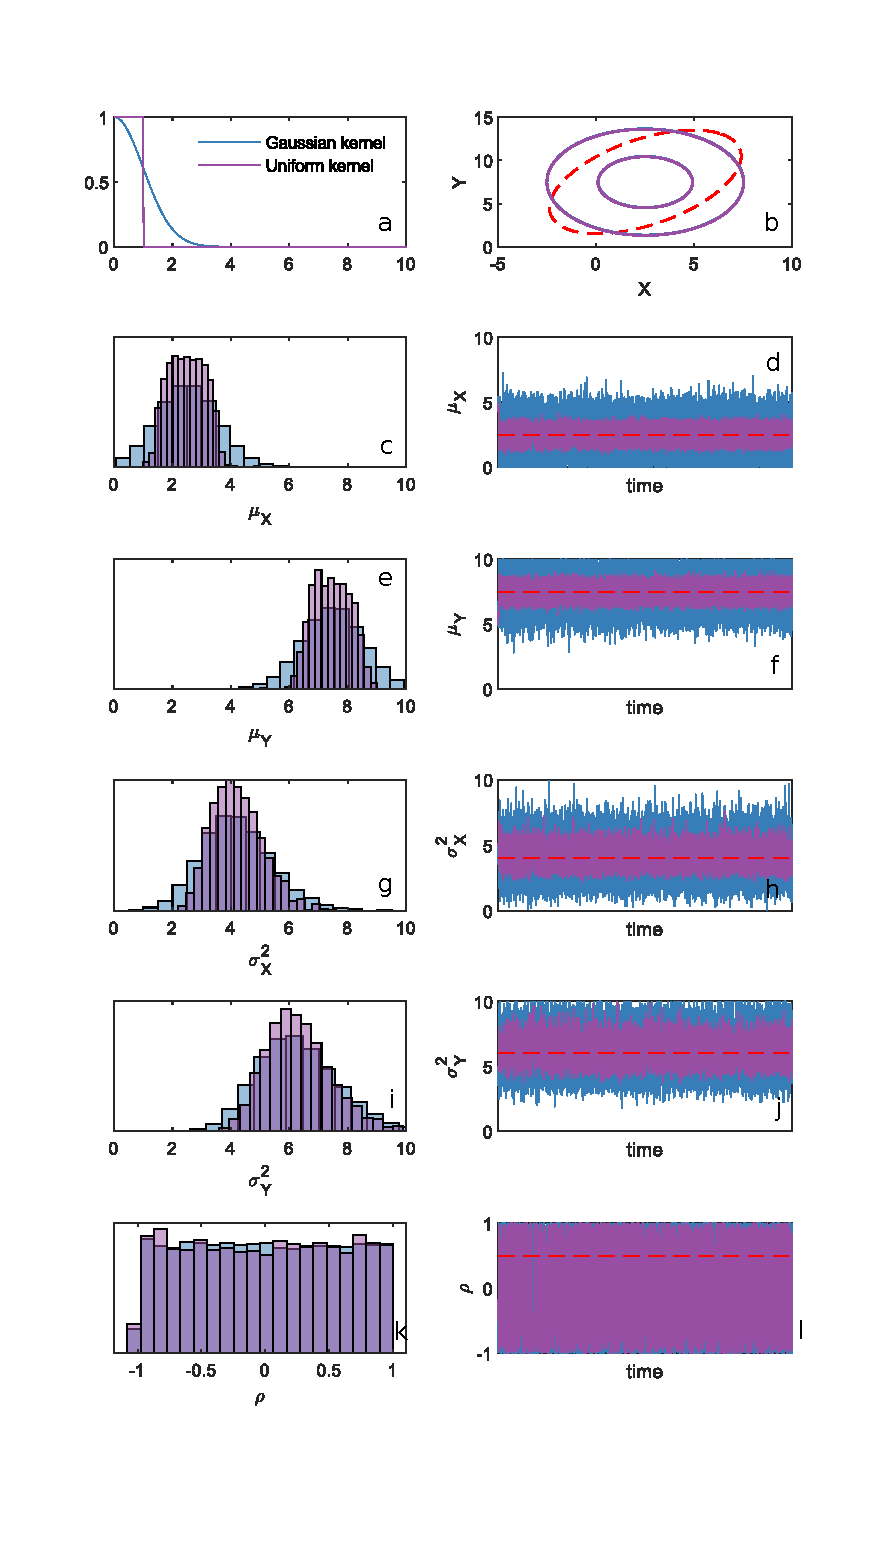
\includegraphics[scale=0.8]{BG1000000.pdf}
	\caption{}
\end{figure}



\section{Toy problem 4: Banana distribution}

As a fourth example we desgin a more challenging problem, one for which there are no imediate and obvious summary statistics and has some degree of dimensionality. Consider we have $n = 1000$ observations from a "banana" distribution, Figure \ref{banana-data}. To define the banana distribution, we start with a 2-dimensional Gaussian distribution:
\begin{equation}
\begin{bmatrix}
x\ y
\end{bmatrix}=\mathcal{N}(\bm{\mu},\bm{\Sigma}),\ \bm{\mu} = \begin{bmatrix}
\mu_X\ \mu_Y
\end{bmatrix}^T,\ \bm{\Sigma} = \begin{bmatrix}
\sigma^2_X & \rho\sigma_X\sigma_Y\\
\rho\sigma_X\sigma_Y & \sigma^2_Y
\end{bmatrix} 
\label{gauss-banana}
\end{equation}
The Gaussian co-ordinates $x$ and $y$ are then twisted to produce a more nonlinear target, $X$ and $Y$, using:
\begin{equation}
X = b_1x
\label{x-banana}
\end{equation}
\begin{equation}
Y = y/a-b_2(b_1^2x^2+b_1^2)
\label{y-banana}
\end{equation}
In total the parameters which define this model are $\bm{\mu}$, $\bm{\Sigma}$ and the banana parameters $\begin{bmatrix}
b_1\ b_2
\end{bmatrix}$. Here the unknown target parameters are $\bm{\mu} = \begin{bmatrix}
0\ 0
\end{bmatrix}^T$.
$\bm{\Sigma} = \begin{bmatrix}
\sigma^2_X & \rho\sigma_X\sigma_Y\\
\rho\sigma_X\sigma_Y & \sigma^2_Y
\end{bmatrix}$ and $\begin{bmatrix}
b_1\ b_2
\end{bmatrix}$ = $\begin{bmatrix}
1\ 1
\end{bmatrix}$. 

\begin{figure}[H]
\centering
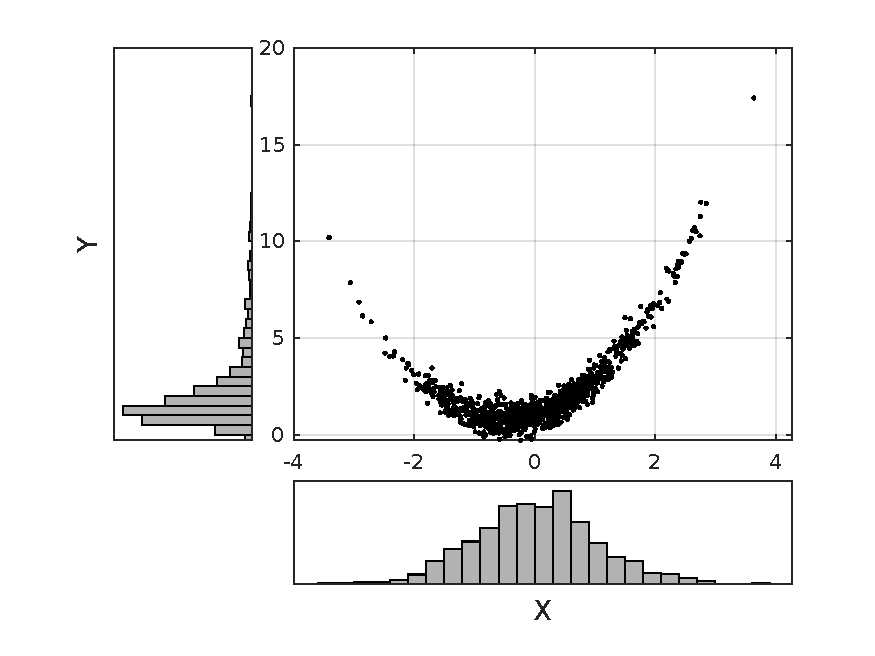
\includegraphics[scale=1]{banana-data.pdf}
\caption{$n = 1000$ observations from the "banana" distribution, analytically defined by equations \ref{gauss-banana}, \ref{x-banana}, \ref{y-banana}. 
This problem is more challenging as there is no immediately apparent sufficient statistics to facilite ABC estimation of the unknown parameters.}
\label{banana-data}
\end{figure}

To proceed with ABC inference under this model we must define a set of reasonably sufficient statistics. In the previous example it was possible to use the sample values for each of the unknown parameter, however, here this proved to be insufficient in a trial run. In the ABC literature summary statistic selection is the focus of technique development and active research. XX and YY have good reveiws of this research area. For this example we heed the advice of \citet{Wood2010}. Firstly, the statsitics have the same role in ABC as the data do in a traditional likelihood. Hence, there is no need for certain statistics to relate to specific parameters any more than there is the need for certain data points to relate to specific parameters. The key is in indenitifying a set of statistics which is senstitive to the scientificaly important and repeatable features of the data, and insensitive to the transient noisey components. \citet{Wood2010} identifies marginal distribution statistics as being a useful first step. The marginal distribution for our banana observations, $X$ and $Y$, are plotted in figure \ref{banana-data}. Here we can see $X$ appears as a regular Gaussian distribution, while $Y$ appears as a skewed-Gaussian distribution. This motivates the choice of marginal statistics for $X$ as the sample mean, $\bar{\mu_X}$, and sample standard deviation, $\bar{\sigma_X}$. While marginal statistics for $Y$ are sample skewness $\bar{\gamma_Y}$, as well as $\bar{\mu_Y}$ and $\bar{\sigma_Y}$. However, this does not capture the "shape" of the joint distribution in 2D dimensions. To capture the bananity of the joint distribution we fit a second degree polynomial to the data, $Y = aX^2 + bX + c$. The co-effecient values $a$, $b$ and $c$ are then used as the summary statistics. For this example we consider this set, $\begin{bmatrix}
\bar{\mu_X}\ \bar{\sigma_X}\ \bar{\gamma_Y}\ \bar{\mu_Y}\ \bar{\sigma_Y}\ a\ b\ c
\end{bmatrix}^T$, to constitute reasonably sufficent summary statistics for the banana distribution. However, these are not perfect, and the effect of using them will be the introduction of some degree of bias into the posterior. \\

% Introduce scaling considerations

Figure YY shows the results of an ABC-MCMC algorithm with a Gaussian kernel and summary statistics as described targeting the banana distribution. For this problem only the Gaussian parameters, $\bm{\mu}$ and $\bm{\Sigma}$ are unknown.\\

The performance of our MCMC algorithm as described by algorithm \ref{ABC-MCMC} depends on the user's ability to choose a suitable proposal distribution $q(.,.)$. If we limit ourselves to a multivariate Gaussian distribution, then we must choose a suitable covariance matrix. If the variance for each parameter is too large then the probability of accepting a proposal will be low, as each step will be erratic and far from the current location. Consider that as the variance $q(.,.) \rightarrow \infty$ we effectively have a Monte Carlo scheme. However, if the variance is too small then the acceptance rate will be very good but algorithm will fail to explore the full parameter space. Hence there is a balance encoded in the selection of the proposal. We desire both a reasonable acceptance and a good exploration of the parameter space. In this way we select a proposal distribution which suits the underlying target distribution. Generally it is simplest to leave the off-diagonal terms in the proposal distribution, the correlations between parameters, unconsidered.\\

However, such a system is not ideal. Selecting an optimal proposal distribution is non-trivial problem. Here we can turn to theoretical developments to guide a better proposal distribution. \citet{gelman1996} show that when the target distribution is Gaussian, an efficient sampler can be constructed by scaling the proposal covariance to $2.4^2/d$, where $d$ is the number of unknown parameters. Until now it has been best to ignore the correlations between parameters. However, these correlations can be important to consider, if there are strong parameter correlations in the posterior then sampling success can be weakened by leaving these set to 0, especially in a high dimensional space and for nonlinear problems. But knowing about these correlations and designing a pre-defined proposal is next to impossible. Ideally the algorithm should be able to learn about the posterior on the fly, and if there are correlations betweeen parameters, adjust accordingly. With this in mind \citet{haario2001} developed Adaptive Metropolis (AM). AM tunes the proposal distribution to the posterior distribution by using the history of the chain generated so far. After some designated time, $t$, the covariance matrix to the proposal distribution, $\bm{\Sigma_q}$, is set to the covariance of the Markov chain so far. 
\begin{equation}
\bm{\Sigma_q} = \text{cov}(\bm{\theta}_1,\dots,\bm{\theta}_t)s + I\upsilon
\end{equation}
Where $s$ is the scaling factor, generally $2.4^2/d$, and $\upsilon$ is a small positive which prevents the covariance from becoming singular. \\

Figure XX plots the effect AM has on a sub-optimal choice for a proposal distribution, and the computational advantage gained from adaption. \\

\begin{figure}[H]
\centering
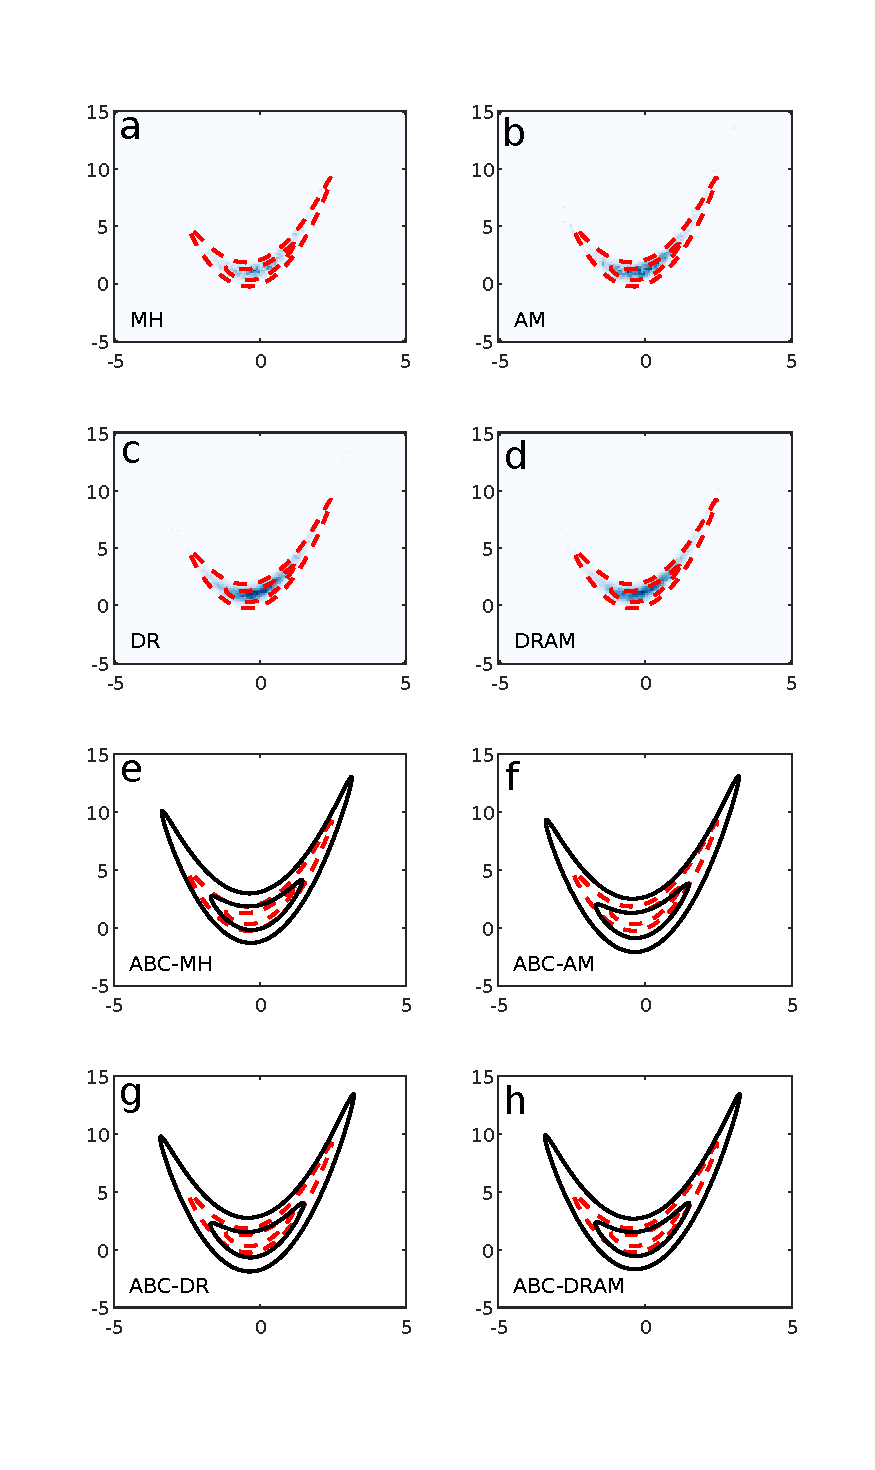
\includegraphics[scale=0.75]{BananaABCvsMCMC.pdf}
\caption{Pdf test}
\end{figure}

\chapter{Synthetic geophysical test}

This chapter will outline a series of experiments which will test the main postulate of this thesis, that ABC can offer some improvement over traditional likelihood based Bayesian inference for geophysics. There are many potential avenues to pursue 'improvement'. For example, ABC opens parameter inference to models which were previously closed. This can be used to compare the solution of parameter inference for a stochastic forward where the data and modelization uncertainty do not conform to a Gaussian, to the solution obtained with the simplifying assumption that the uncertainty is Gaussian. This may constitute an improvement in accuracy if it is shown that the ABC solution is significantly different from the analytical Gaussian solution. Instead of pursuing this angle, here I focus explicitly on improving the speed of optimization relative to a general form MCMC sampler. Probabilistic methods which rely on Monte Carlo and MCMC are computationally expensive due to the need to compute the forward at every iteration of the algorithm. As a result the scale of the problems which are computationally tractable is limited. If our limits of understanding about the Earth are to be pushed then it is necessary to develop methods which can tackle large scale problems which are fundamentally defined by solution spaces with uncertainty due to trade-offs between parameters, uncertainty in the experimental data and uncertainty in the modelization process. In this context there is great need for methods which can efficiently find, and then define regions of high probability in very sparse parameter spaces. \par

Here I seek to use the information available by 'opening' the likelihood within each forward simulation to drive improved optimization with ABC, a method which can take into account the full scope of uncertainty in the resulting solution. In this way I abandon the mathematical generality of the applied sampling algorithm in pursuit of one purpose built for the information available within the problem. \par

As with the previous chapter, the code to produce all figures in this section can be found at \url{https://github.com/tomconnell/approximate-bayesian-tomography}.\par


\section{Crustal density inversion}

As a first experiment, I consider an inversion for crustal density (\rho) with a vertical gravity anomaly dataset (\Delta g) for a 2D discretized subsurface \citep[p.184-195,378]{blakely1996}. The dimensionality of the parameter space is kept modest, a 8x4 grid, with an observed data point above each column. The grid is defined over a 160 $km$ by 40 $km$ area. The parameter space is bounded between 2-3.5 $g/cm^3$, the limits for which \citet{Brocher2005} define an empirical relationship between density and compressional-wave velocity ($V_p$). This relationship will be used in the next section for a joint inversion. The true model is kept smooth, to allow a prior term, $p(\bm{\theta})$, to be set for smoothness which will limit the inversion to a unique solution. The definition for smoothness is:
\begin{equation}
\text{log}\big(p(\bm{\theta})\big) = \sum_{i = 1}^{N} \Big(\sum_{j} (\rho_i - \rho_j)^2\Big)
\end{equation}
where $j$ is a describes all blocks in immediate contact with the given block, $i$. The edge effect for the 2D subsurface grid is compensated by adding the vertical gravity anomaly which will result from extending the grid by a width of one on both sides, tripling the total domain width, with a density which is the average of the parameter space, 2.75 $g/cm^3$.




\section{Crustal density joint inversion}

% Conclusion
%------------------------------------------------------
% QUOTE
% If you really feel like adding a quote
% to your page, uncomment out the following.
%------------------------------------------------------
%\begin{savequote}[45mm]
%When theory and experiment agree, 
%that is the time to be especially suspicious. 
%\qauthor{Niels Bohr}
%\end{savequote}
%------------------------------------------------------
% QUOTE
% If you really feel like adding a quote
% to your page, uncomment out the previous.
%------------------------------------------------------


\chapter{Conclusion}

Not a very interesting conclusion, however you'll need one for your thesis.


\makeatletter
\let\@makechapterhead\old@makechapterhead
%---------------------------------------------------------- 
% BACK
% list of symbols / references / index etc
%---------------------------------------------------------- 
\backmatter

% your thesis may not need this, so comment out or delete the following line
%\chapter{List of Symbols}

% please change this list to suit your thesis

The following list is neither exhaustive nor exclusive, but may be helpful.
\begin{list}{}{%
\setlength{\labelwidth}{24mm}
\setlength{\leftmargin}{10mm}}
\item $\mathcal{M} \equiv$ a causative physical model defined by a set of known/unknown parameters
\item $\bm{\theta} = \{\theta_1,...,\theta_N\} \equiv$ unknown parameters to the model $\mathcal{M}$
\item $\bm{\theta'} = \{\theta'_1,...,\theta'_N\} \equiv$ a specified set of parameters to the model $\mathcal{M}$
\item $\bm{y} = \{y_1,...,y_m\} \equiv$ set of observed experimental data
\item $\bm{y'} = \{y'_1,...,y'_m\} \equiv$ set of simulated data from $\mathcal{M}(\bm{\theta'})$
\item $\mathcal{L}(\bm{m}) \equiv$ the likelihood 
\end{list}



% Bibliography, in BibTeX format (the references.bib file)
\bibliographystyle{apalike}
\linespread{1}\selectfont
\bibliography{abc}


%---------------------------------------------------------- 
% APPENDICES
% include chapters as needed (will be numbered differently)
%---------------------------------------------------------- 
%\appendix
\chapter{Supplementary material}
\label{supplementary-material}
\newpage
\begin{figure}[H]
	\centering
	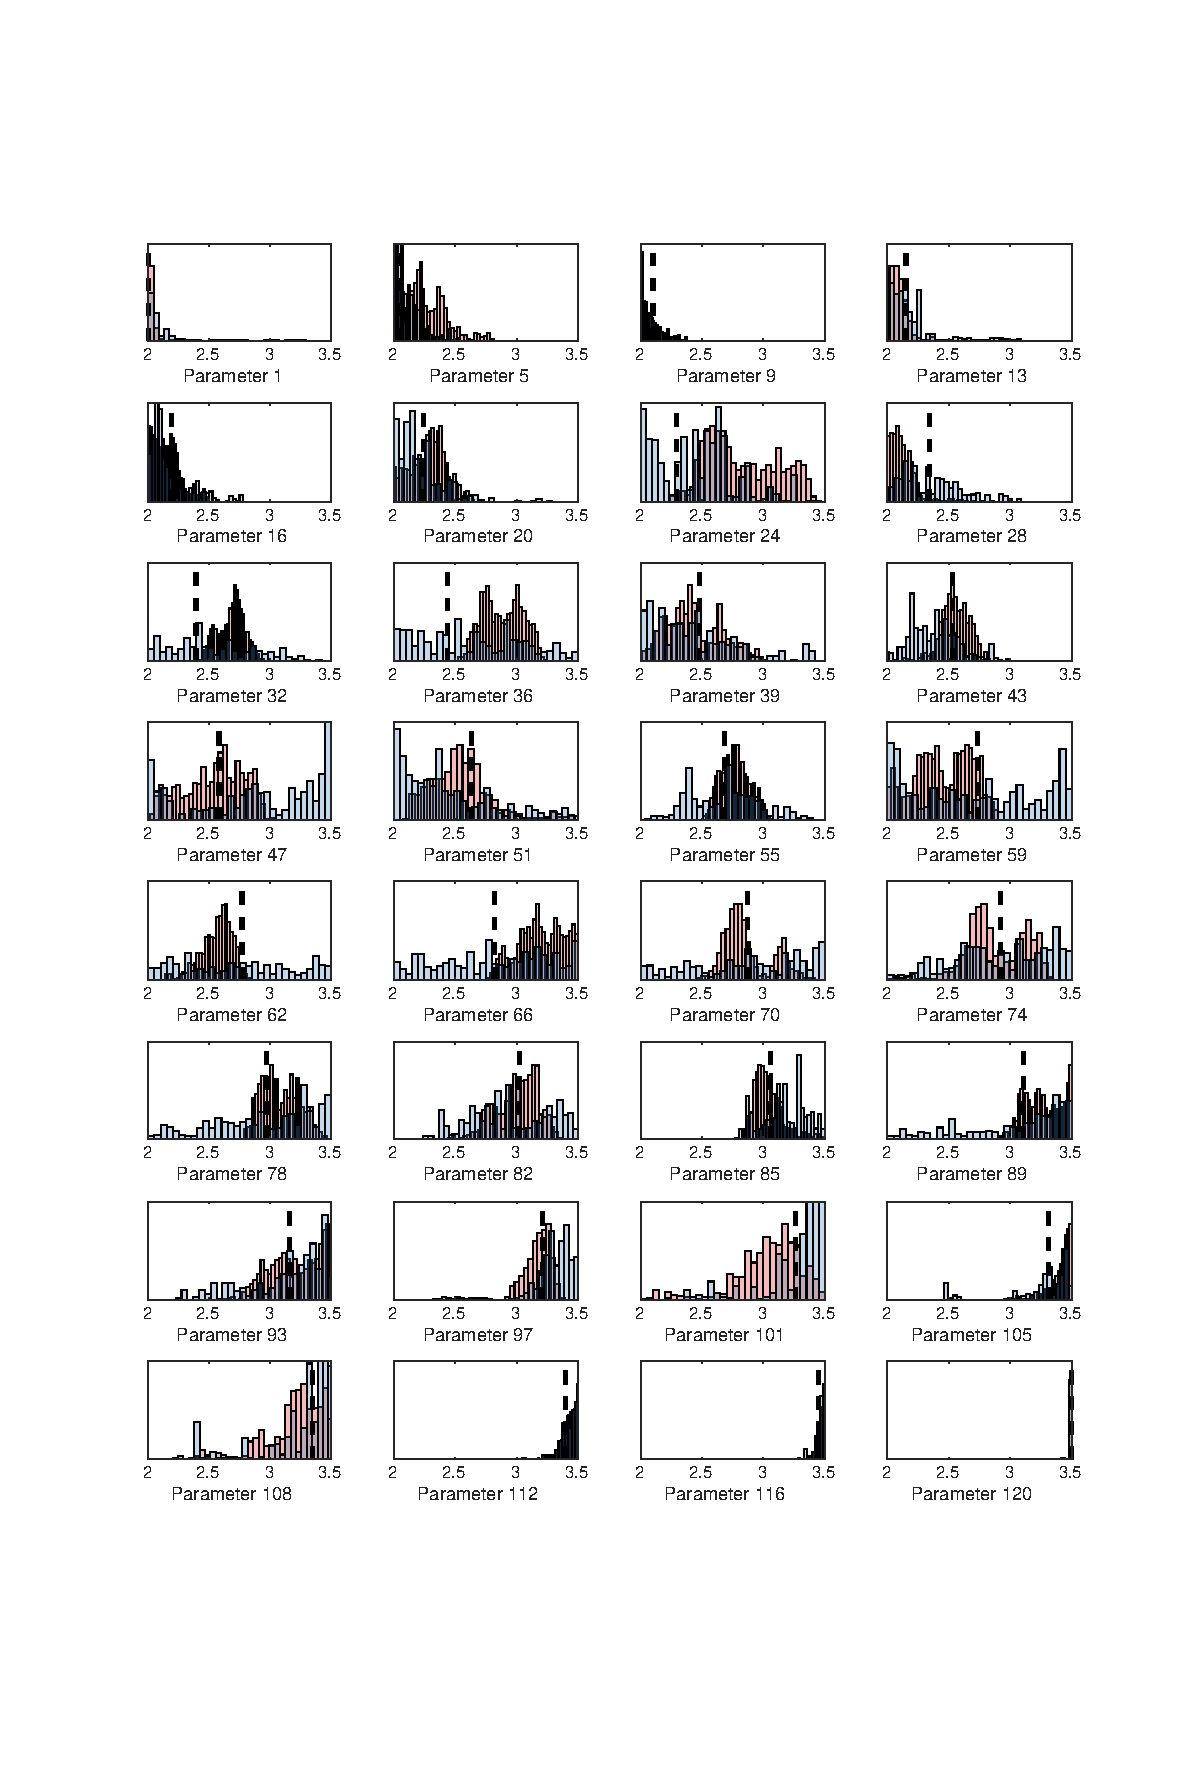
\includegraphics[scale=0.7]{joint-hist-reg-tol.pdf}
	\caption{A comparison of the marginal ABC posterior (blue), sampled by the diagnostic ABC joint inversion, and the analytically defined posterior (red), sampled by MCMC, for a subset of the parameter space. This is the PDF which underlies the experiment in section \ref{SGE} and figures \ref{comparison-trunc}, \ref{grav-trunc} and \ref{tom-trunc}. The tolerance here is $\epsilon = \vec{1}\cdot0.1$. The black dashed lines marks the `true' parameter values from figures \ref{true-model-large-grav} and \ref{true-model-tom}. This ABC posterior can be compared to the ABC posterior for the same problem with $\epsilon = \vec{1}\cdot0.05$, figure \ref{pdf-half-tol} and $\epsilon = \vec{1}\cdot0.025$, figure \ref{pdf-quart-tol}. The parameters are numbered down column, starting with `1' in the top left corner (figure \ref{true-model-large-grav}).}
	\label{pdf-reg-tol}
\end{figure}

\begin{figure}[H]
	\centering
	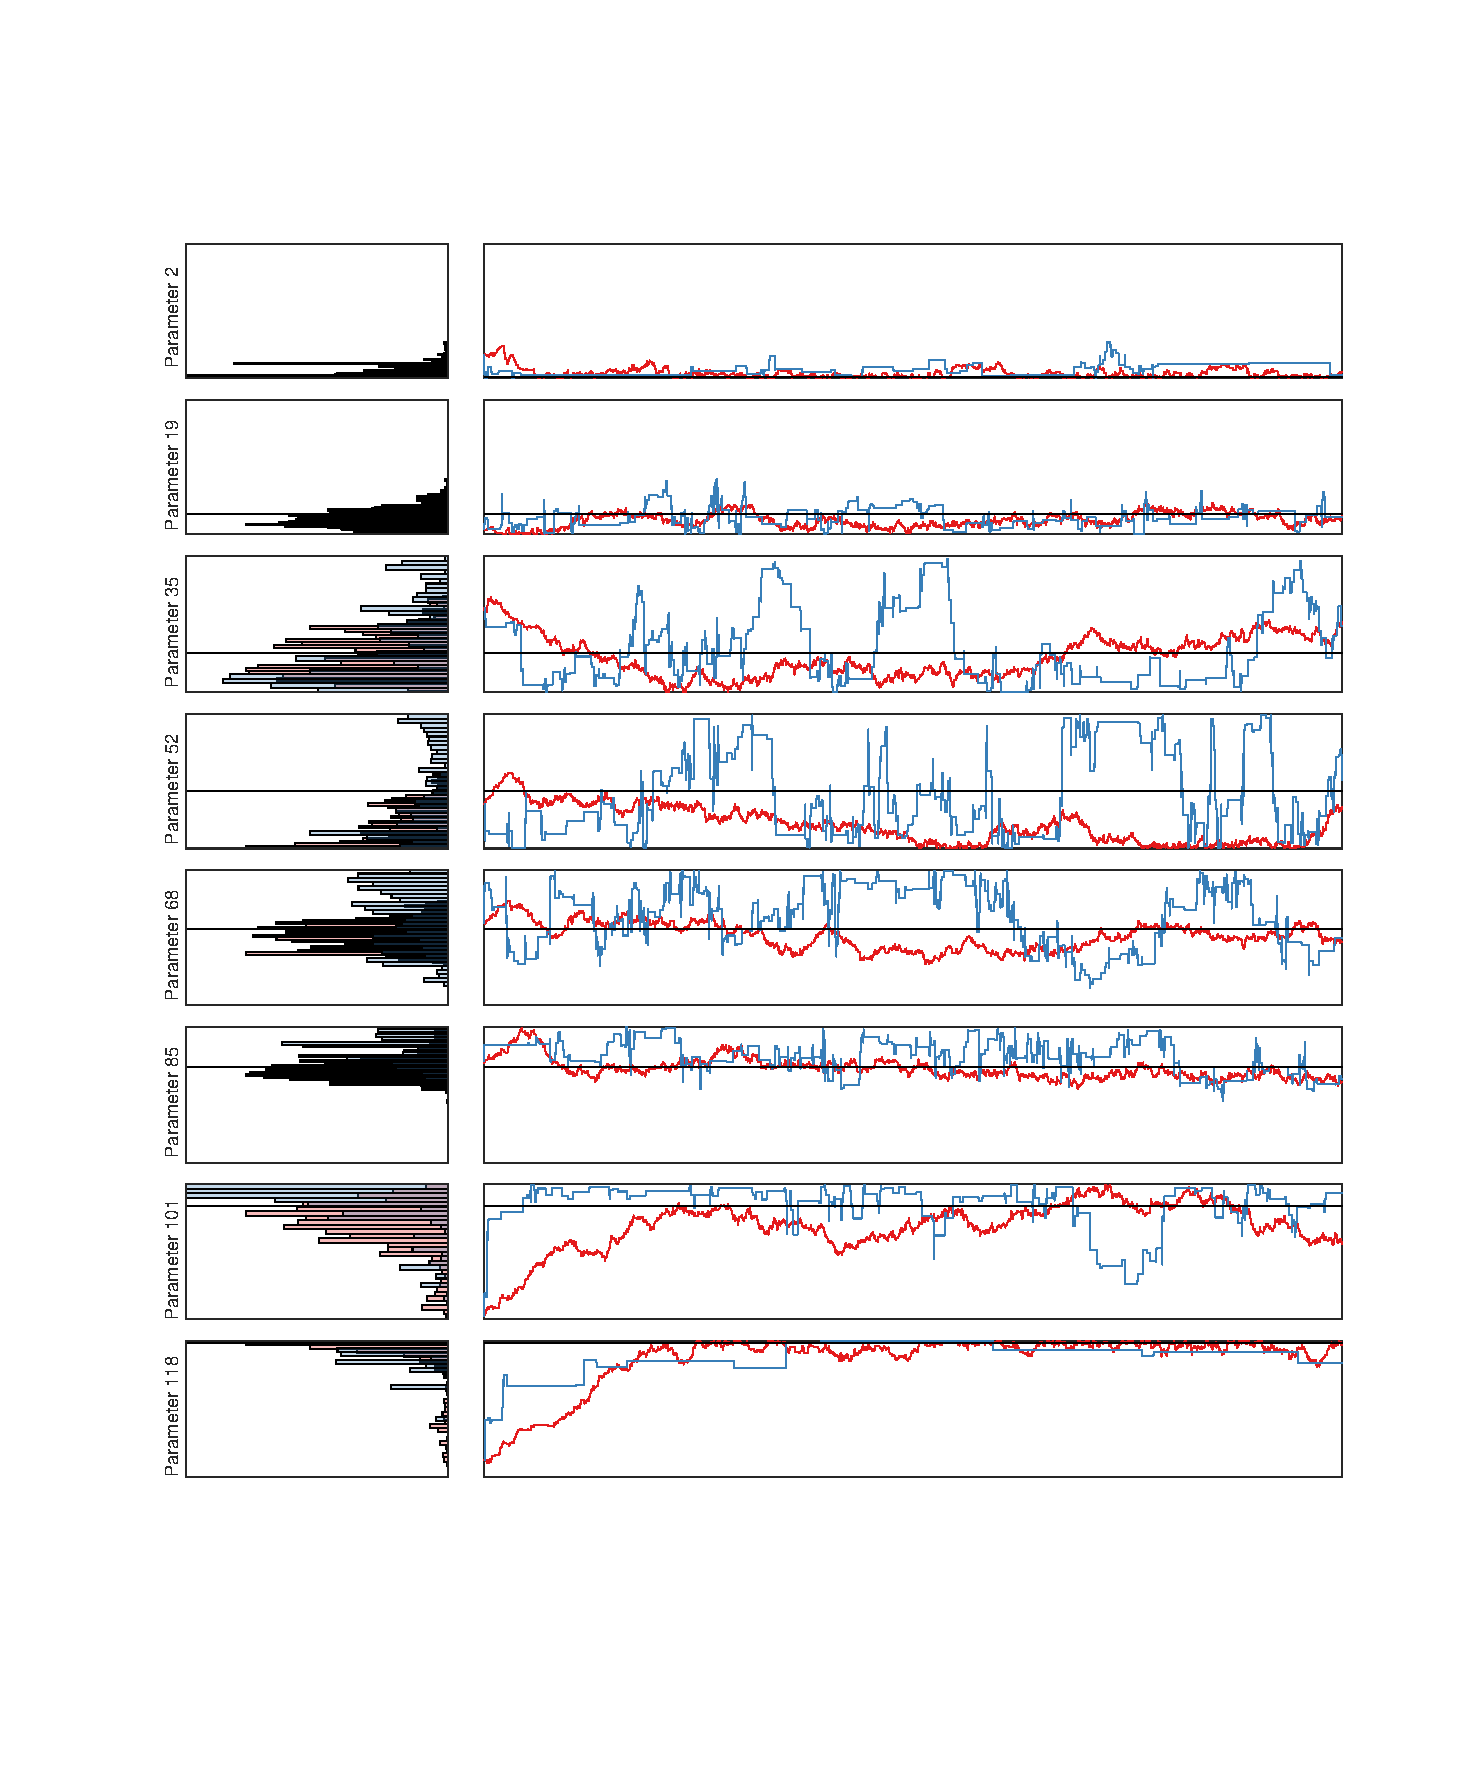
\includegraphics[scale=0.7]{marginals-reg-tol.pdf}
	\caption{A comparison of Markov chain traces for the sampling of the ABC (blue) and analytically-defined (red) posteriors undertaken in section \ref{SGE}. The Markov chains are both of length 100,000. This figure is limited to a subset of 8 parameters out of the 120 total unknowns. The marginal histograms associated with each chain are also displayed. The black line marks the `true' parameter values from figures \ref{true-model-large-grav} and \ref{true-model-tom}. The parameters are numbered down column, starting with `1' in the top left corner (figure \ref{true-model-large-grav}).}
	\label{marginal-reg-tol}
\end{figure}

\begin{figure}[H]
	\centering
	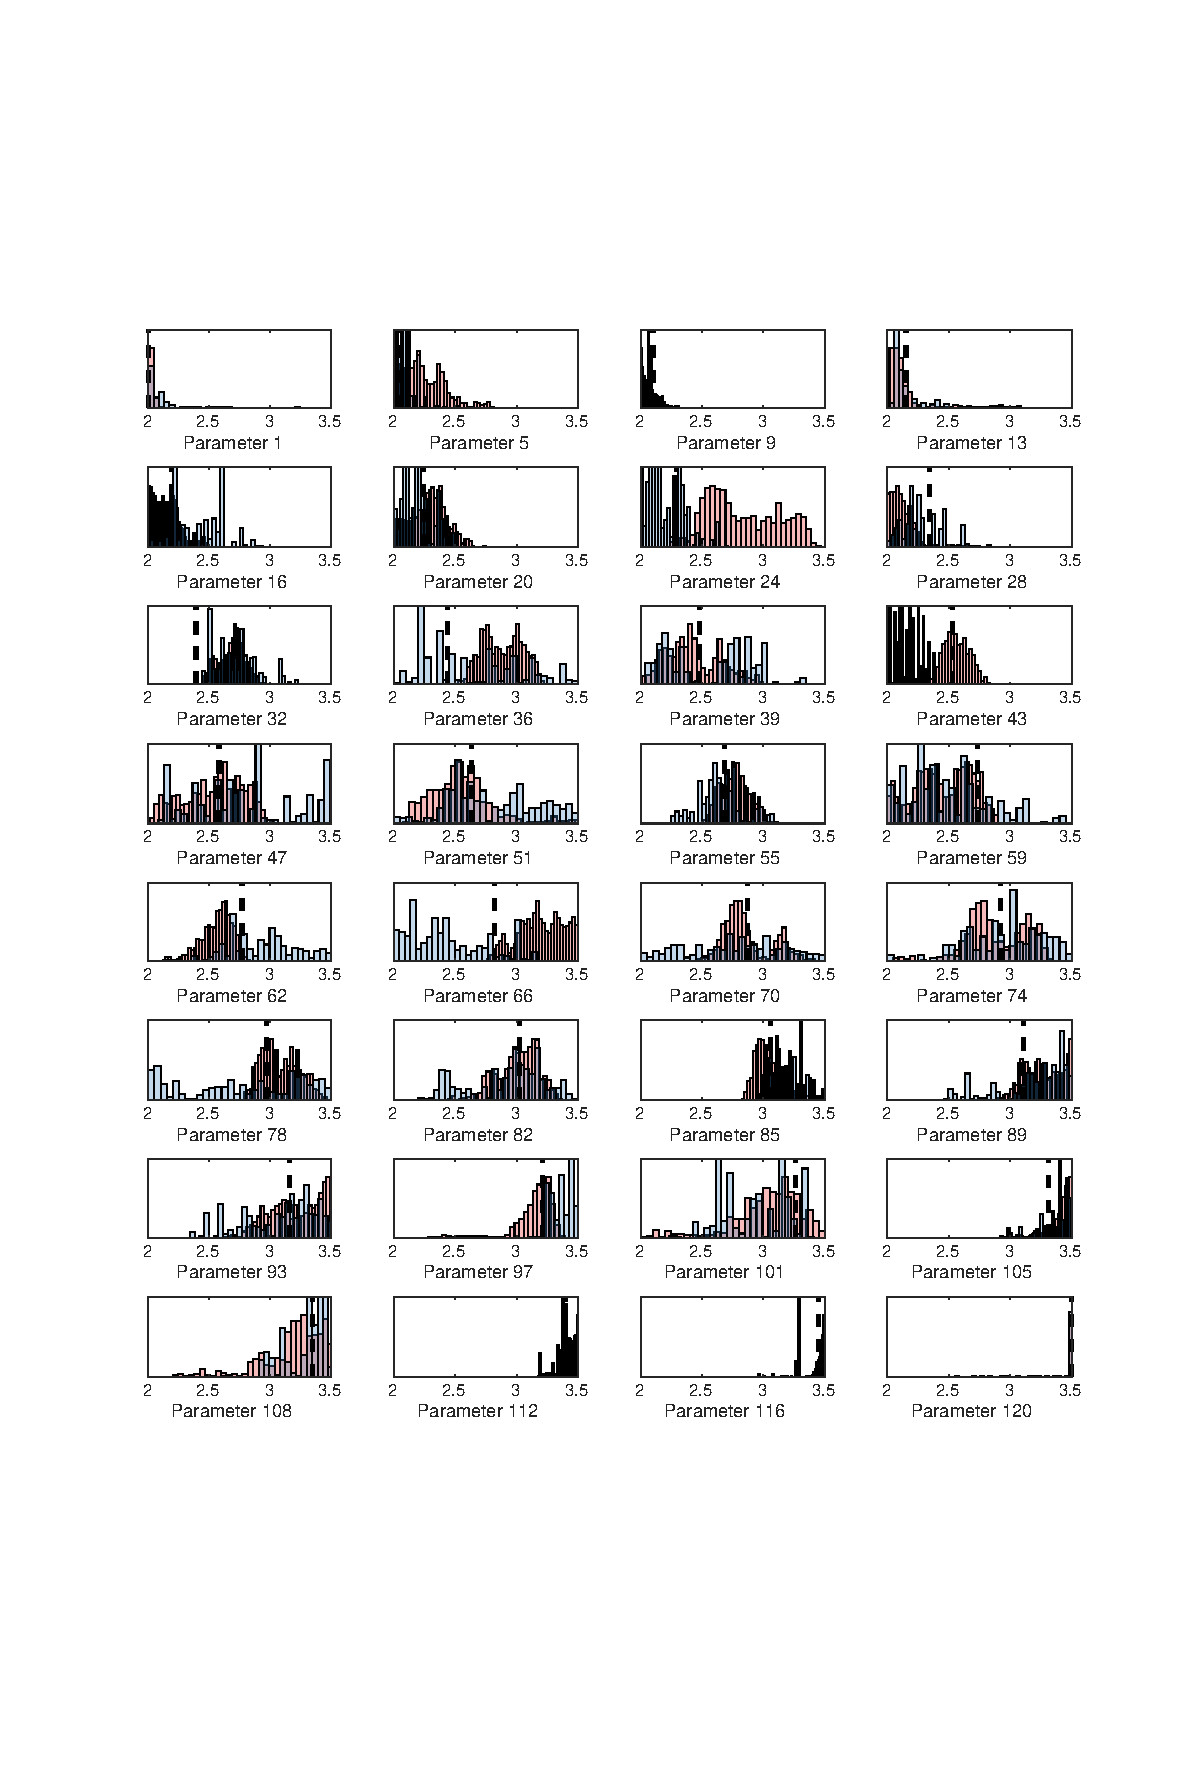
\includegraphics[scale=0.65]{half-tol-joint-hist.pdf}
	\caption{A comparison of the marginal ABC posterior (blue), sampled by the diagnostic ABC joint inversion, and the analytically defined posterior (red), for a repetition of the experiment in section \ref{SGE} with a lower tolerance in the ABC likelihood approximation $p(\bm{S}(\bm{y})|\bm{S}(\bm{y^*},\bm{\theta}))$. The tolerance here is $\epsilon = \vec{1}\cdot0.05$, half the tolerance of the original experiment documented in section \ref{SGE}. The black dashed lines marks the `true' parameter values from figures \ref{true-model-large-grav} and \ref{true-model-tom}. This ABC posterior can be compared to the ABC posterior for the original experiment, figure \ref{pdf-half-tol} and an ABC posterior with $\epsilon = \vec{1}\cdot0.025$, figure \ref{pdf-quart-tol}. The sampling acceptance rate of the ABC posterior documented in this figure is 2.635\%, and the auto-correlation time ($\tau$) is 7892, figure \ref{comparison-quart-tol}.}
	\label{pdf-half-tol}
\end{figure}

\begin{figure}[H]
	\centering
	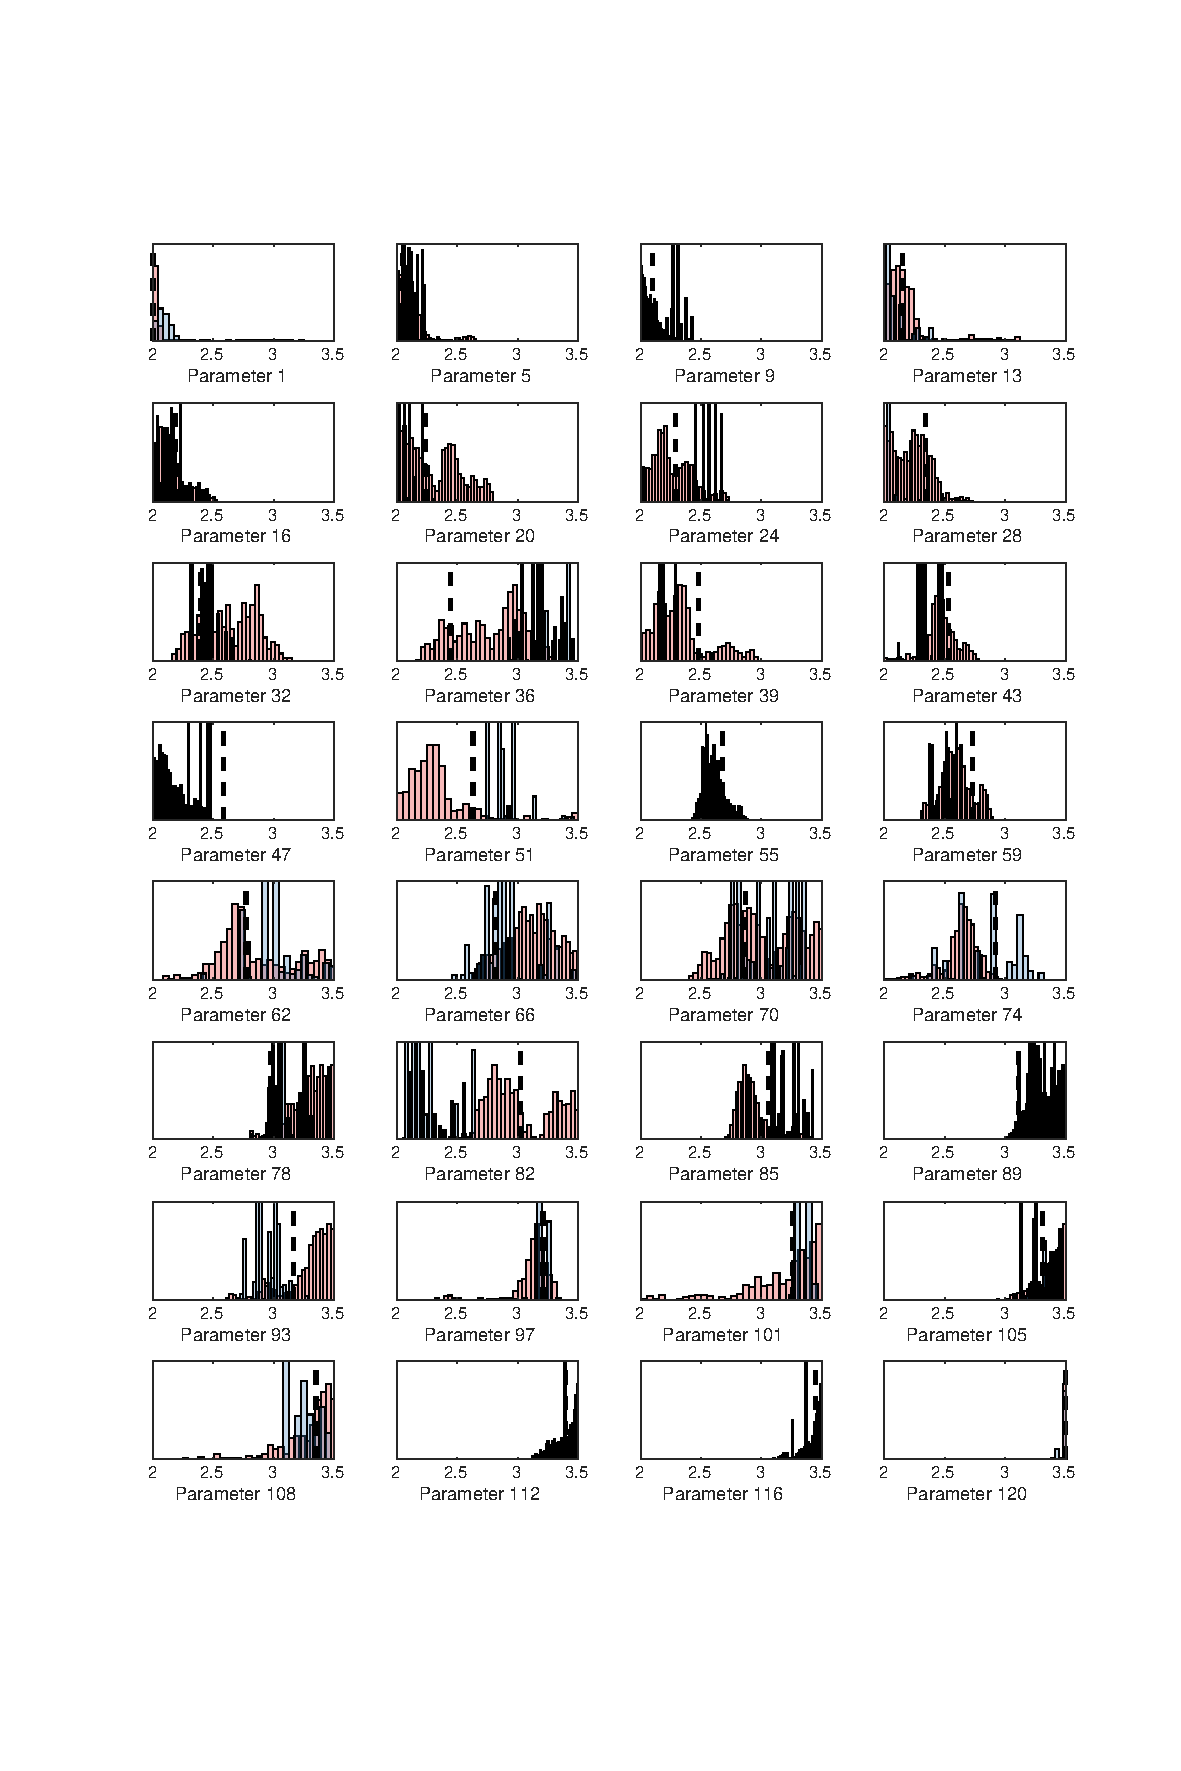
\includegraphics[scale=0.7]{quart-tol-hist.pdf}
	\caption{}
	\label{pdf-quart-tol}
\end{figure}

\begin{figure}[H]
	\centering
	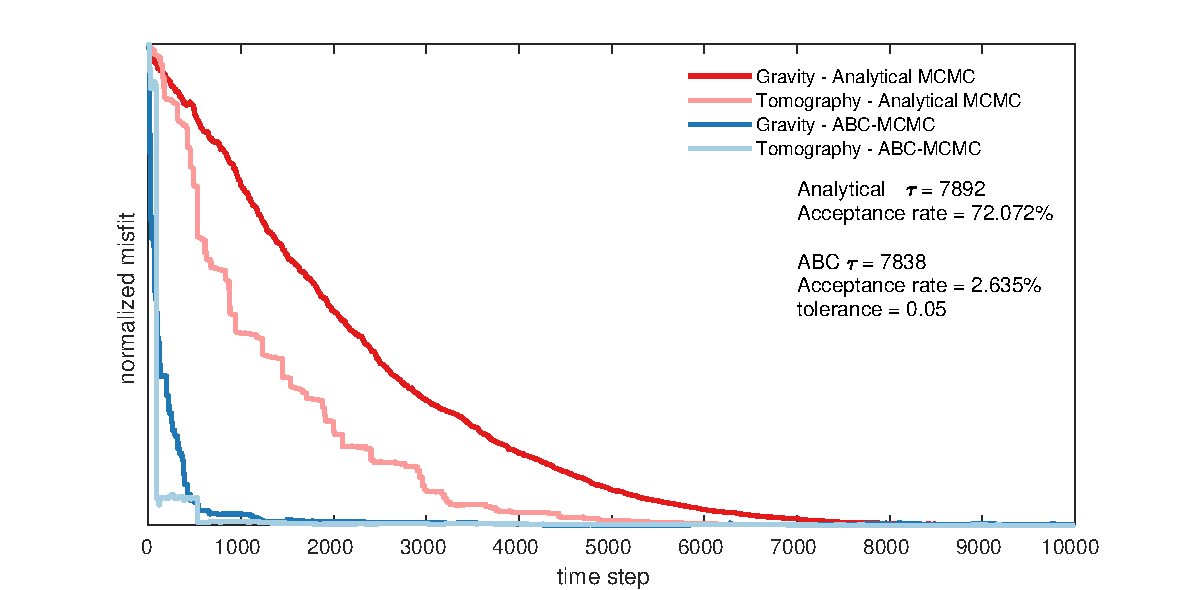
\includegraphics[scale=0.8]{half-tol-comparison.pdf}
	\caption{}
	\label{comparison-half-tol}
\end{figure}

\begin{figure}[H]
	\centering
	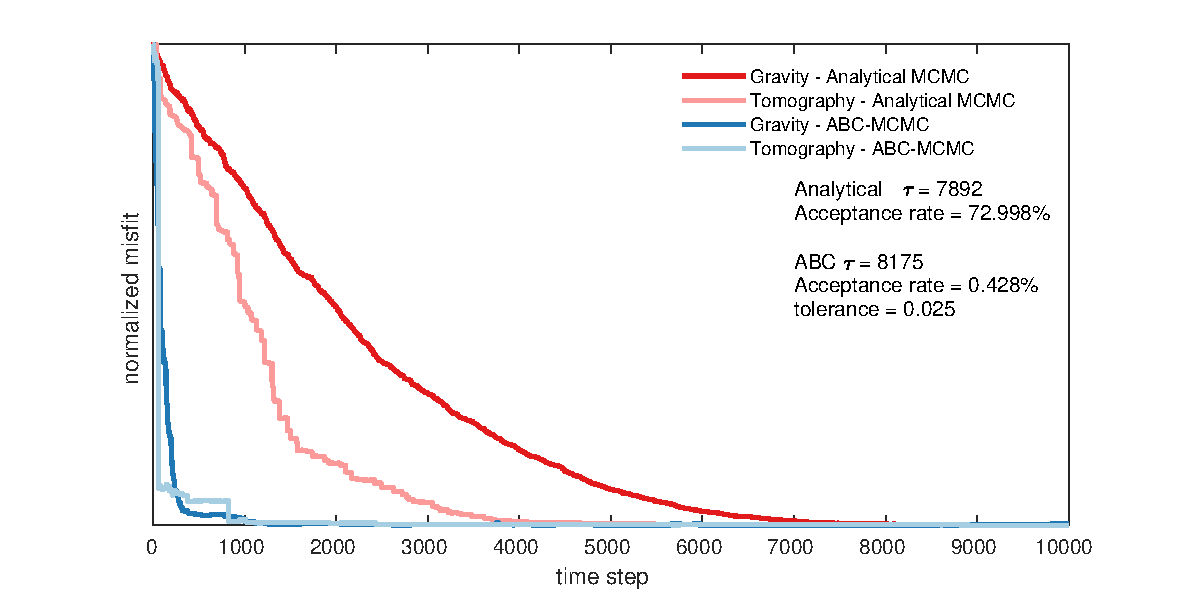
\includegraphics[scale=0.8]{quart-tol-comparison.pdf}
	\caption{}
	\label{comparison-quart-tol}
\end{figure}

\begin{figure}[H]
	\centering
	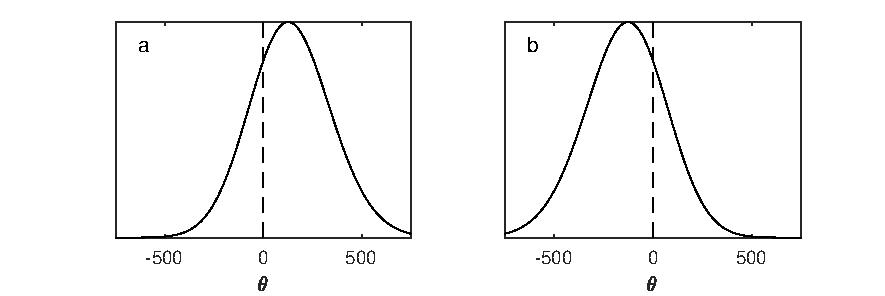
\includegraphics[scale=1.1]{skew_updates.pdf}
	\caption{The skew Gaussian proposal distributions which can be used to positively or negatively bias the parameter update as an alternative to the truncated Gaussian distribution, figure \ref{updates}. The positively skewed distribution (a) is used when the parameter values are deemed too low. The negatively skewed distribution (b) is used when the parameter values are deemed too high. During application the distributions are centered on the current chain and $\omega = 250$.}
	\label{skew-updates}
\end{figure}

\begin{figure}[H]
	\centering
	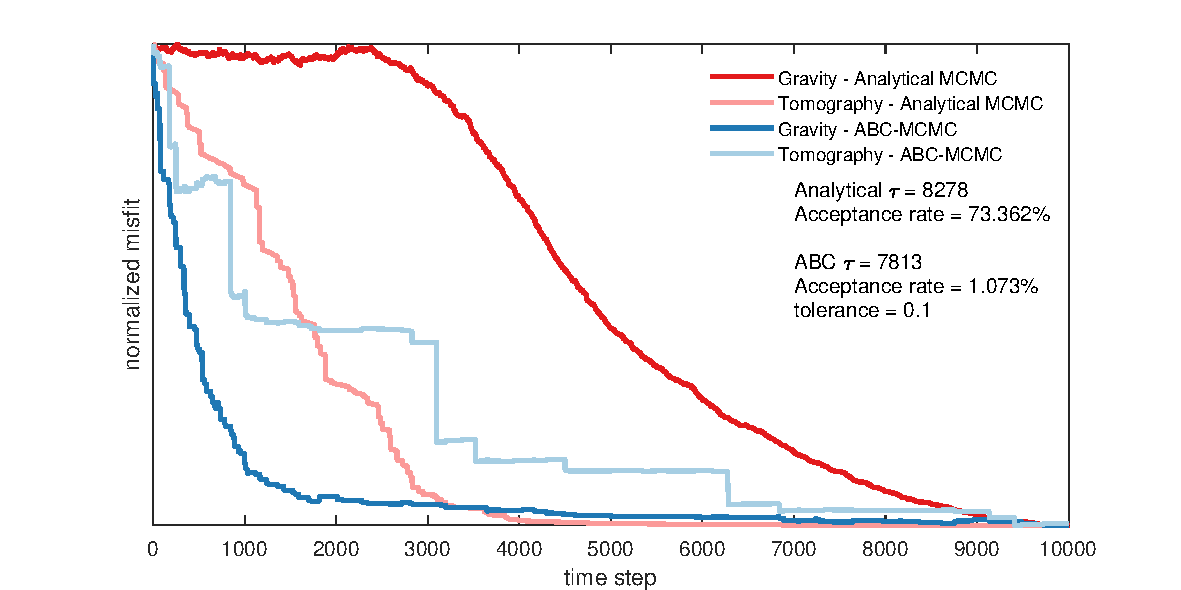
\includegraphics[scale=0.8]{comparison-skew.pdf}
	\caption{Skew Gaussian scheme. The normalized misfit of the chain state during the initial phase (first 10,000 steps) for both datasets, $\Delta g$ and $\Delta t$, and for both methods, an analytically defined posterior sampled by MCMC and ABC-tomography. The `true model' and observed data is plotted in figure \ref{true-model-large-grav} and \ref{true-model-tom}. The increase in the rate of convergence to a low misfit model under ABC-tomography is a result of dynamically selecting, localizing and directly the update at each time step in the Markov chain. The details of the full chain run (100,000 time steps), are also displayed on the figure. $\tau$ is the integrated auto-correlation time. The mean marginal models from ABC-tomography using skew Gaussian updates is plotted in figure \ref{grav-skew} and \ref{tom-skew}.}
	\label{comparison-skew}
\end{figure}

\begin{figure}[H]
	\centering
	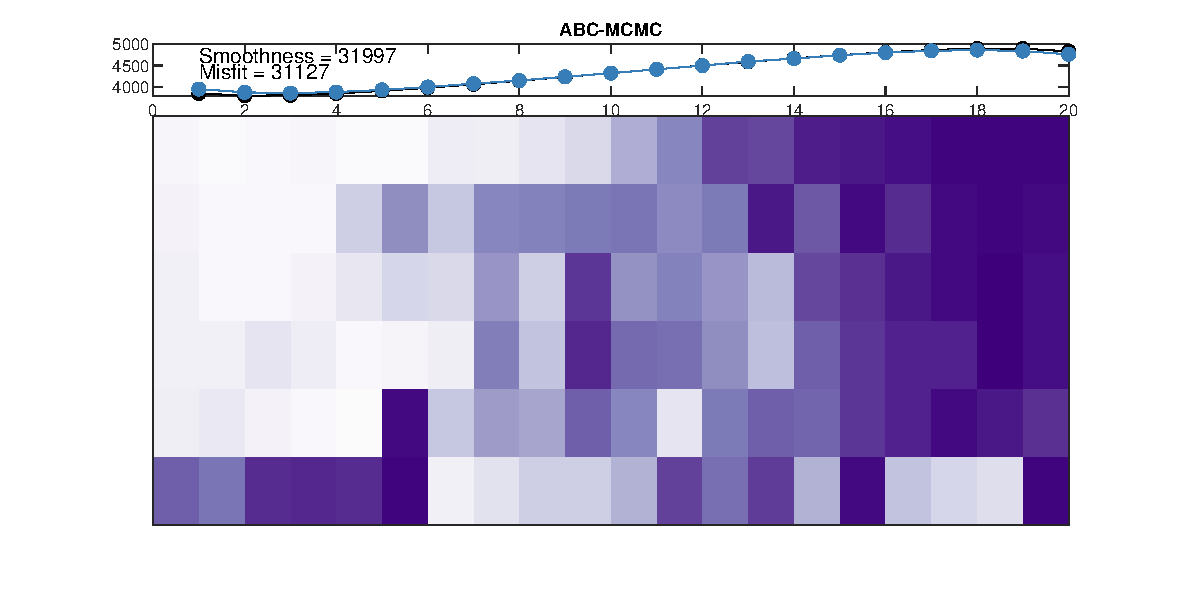
\includegraphics[scale=0.7]{abc_im-skew.pdf}
	\caption{Skew Gaussian scheme. The mean of the marginal ABC posterior, $p_{ABC}(\bm{\theta}|\bm{S}(\bm{y}))$, targeting the `true model' and observed data of figure \ref{true-model-large-grav}. The simulated data generated by this `solution', is plotted, blue, compared to the observed data, black. The misfit during the initial phase for this chain is plotted in figure \ref{comparison-skew}. The corresponding mean marginal $V_p$ model is plotted in figure \ref{tom-skew}.}
	\label{grav-skew}
\end{figure}

\begin{figure}[H]
	\centering
	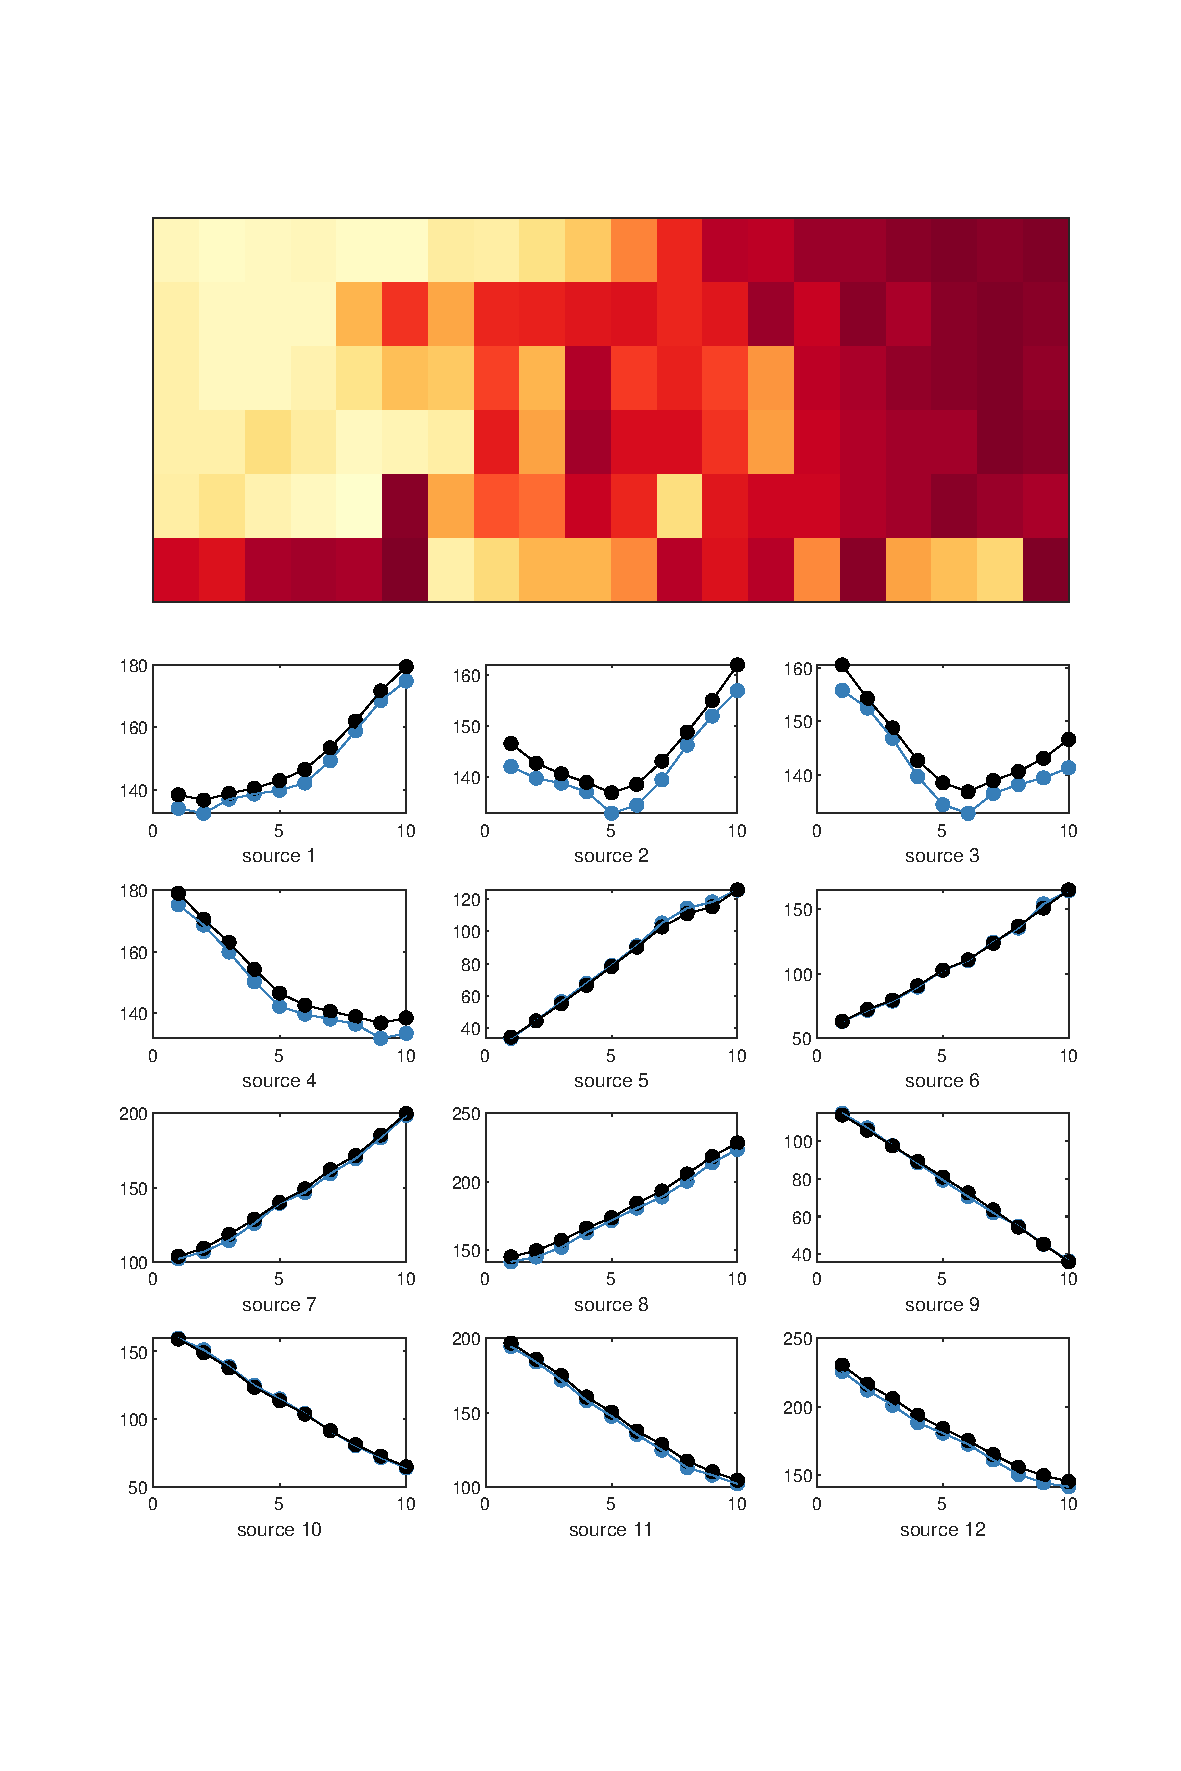
\includegraphics[scale=0.7]{abc-skew.pdf}
	\caption{Skew Gaussian scheme. The mean of the marginal ABC posterior, $p_{ABC}(\bm{\theta}|\bm{S}(\bm{y}))$, targeting the `true model' and observed data of figure \ref{true-model-tom}. The simulated data generated by this `solution', is plotted, blue, compared to the observed data, black. The misfit during the initial phase for this chain is plotted in figure \ref{comparison-skew}. The corresponding mean marginal $\rho$ model is plotted in figure \ref{grav-skew}.}
	\label{tom-skew}
\end{figure}




\end{document}
